\documentclass[a4paper]{instrumentacao}

\usepackage{etoolbox}
\usepackage{float}

\newtoggle{attachments}
\toggletrue{attachments}

\extrafloats{100}

\graphicspath{
	{../Resources/Images/}
	{../Resources/Mathematica/images/}
	{../Resources/MATLAB/images/}
}

\title{Simulação e Experimentos com Células de Cargas}
\author{Rogiel Sulzbach \and Rodrigo de Castro Silveira}
\startdate{02/05/2016}
\finishdate{30/05/2016}
\emails{
	\emailaddress{R.J.S.}{rogiel@rogiel.com},
	\emailaddress{R.C.S.}{csilveira.rodrigo@gmail.com}
}

\resume{}
\abstract{} 
\keywords{célula de carga, experimento, extensômetro, ponte de Wheatstone, SOLIDWORKS, strain gage, torquímetro}
\institute{Universidade Federal do Rio Grande do Sul, Departamento de Engenharia Elétrica, Curso de Engenharia Elétrica, Instrumentação A, Prof. Dr. Alexandre Balbinot}

\headertext{Extensometria}

\begin{document}
\fontsize{12pt}{16pt}\selectfont
\maketitle

\todo{Resumo}

\chapter{Introdução}

Nesta atividade de laboratório foram feitas várias atividades de laboratório utilizando sensores do tipo extesômetro. Um extensômetro é um sensor resistivo cuja resistência elétrica varia com a deformação mecânica do sensor. A Figura \ref{fig:intro-extensometro} apresenta um extensômetro do tipo grade:

\begin{figure}[H]
\center
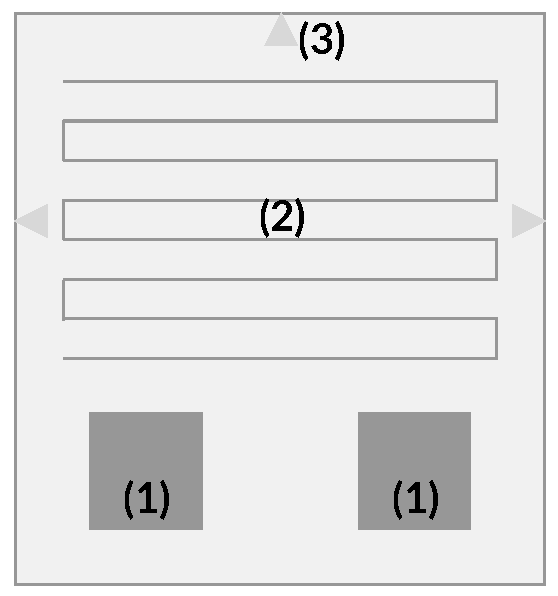
\includegraphics[width=0.5\textwidth]{ExtensometroGrade.pdf}
\caption{Desenho simplificado de um extensômetro do tipo grade}
\label{fig:intro-extensometro}
\end{figure}

\todo{trocar figura do extensômetro na posição correta}

\noindent onde (1) representa os \textit{pads} de conexão elétrica do sensor, (2) é a grade do sensor e (3) são os indicadores de alinhamento do sensor. Este tipo de extensômetro é dito como uniaxial pois deformações fora do seu eixo principal são insignificantes perto da variação de resistência elétrica devido à deformações ao longo do seu eixo principal.

Conforme apresentado na Figura \ref{fig:intro-extensometro} a grade do sensor (2) é composta por um material condutor com uma resistência elétrica característica. Uma vez que o sensor esteja cimentado (colado) sobre uma superfície deformações na superfície se propagam como deformação do sensor que deformam a grade. Deformações na grade causam pequenas alterações (na ordem de $10^{-6} \Omega$) na resistência elétrica do sensor. Com um circuito elétrico de condicionamento adequado, estas pequenas variações de resistência elétrica do sensor podem ser medidas e quantificadas em valores de deformação mecânica.

Os indicadores de alinhamento do sensor (3) conforme apresentados na figura \ref{fig:intro-extensometro}, indicam o ponto de maior sensibilidade do sensor, isto é, onde há a maior variação de resistência elétrica para uma mesma deformação.

O extensômetro pode ser modelado matematicamente de forma simplificada pela Equação \ref{eq:intro-extensometro}:

\begin{equation}
	\frac{\Delta R}{R_0} = k \frac{\Delta l}{l_0} = k\epsilon
	\label {eq:intro-extensometro}
\end{equation}

\noindent onde $\Delta R/R_0$ é a variação relativa de resistência elétrica do sensor referente ao seu valor inicial de repouso (ou nominal) $R_0$, $\Delta l/l_0$ é a deformação mecânica relativa do sensor referente ao seu valor inicial de repouso (ou nominal) $l_0$ também definida como $\epsilon$ e $k$ é uma constante que define a relação entre variação de resistência elétrica e deformação do sensor, conhecido como fator \textit{gage}.

Dessa forma, é possível relacionar a deformação mecânica da grade do sensor com a variação de resistência elétrica do sensor. Como a variação de resistência elétrica é muito baixa (ordem de $10^{-6}$) para que seja possível medir esta variação é necessário que se utilize um circuito de condicionamento de qualidade. Uma topologia muito comum é a utilização da ponte de Wheatstone, que dá origem a 3 montagens comuns com extensômetros: 1/4 de ponte, meia ponte e a ponte completa.

Este relatório versará sobre experimentos utilizando células de carga, onde será levantada a função de transferência experimental para uma célula de carga comercial da HBM e outra célula de carga não-comercial feita com uma simples barra de alumínio e extensômetros cimentados sobre a barra que será validado utilizando um modelo computacional simulado. Adicionalmente foi levantada a função de transferência experimental de um torquímetro disponível no laboratório.

Como a variação de resistência elétrica em extensômetros é observada em um valor tão baixo (ordem de $\mu\Omega$), o circuito de condicionamento é fundamental e portanto uma breve análise em circuitos de condicionamento será feita.

\chapter{Metodologia Experimental}
Nestes experimentos de laboratório foi utilizado o software Wolfram Mathematica 10.4.0 da Wolfram Research, Inc. para realizar todos os cálculos no computador utilizando precisão do tipo MachinePrecision\cite{mathematica-numerial-precision} onde a precisão dos números de ponto flutuante respeitam os critérios impostos pelo processador (64 bits, precisão dupla) que implementam o padrão IEEE de ponto flutuante, possuem um "Épsilon de Máquina", o menor valor que somado a 1 retorna um valor diferente de 1, isto é, não causa arredondamento \cite{wikipedia-epsilon}, de $2^{-52}$, ou seja, na ordem de $10^{-16}$ e podem, portanto, serem desprezados perante a resolução de todos os outros instrumentos utilizados no experimento. Adicionalmente, quando possível, os cálculos foram realizados de forma simbólica com substituição numérica no final. Os scripts utilizados para cálculo estão anexados ao fim do documento, na Página \pageref{ch:attachments}.

Para a realização de simulações mecânicas do modelo computacional 3D foi utilizado o software SOLIDWORKS 2016 SP2 desenvolvido pela Dassault Systèmes SolidWorks Corp.

\section{Ponte de Wheatstone}

Na Figura \ref{fig:celula-comercial-circuito} está apresentado o esquemático elétrico de uma ponte de Wheatstone:

\begin{figure}[H]
\center
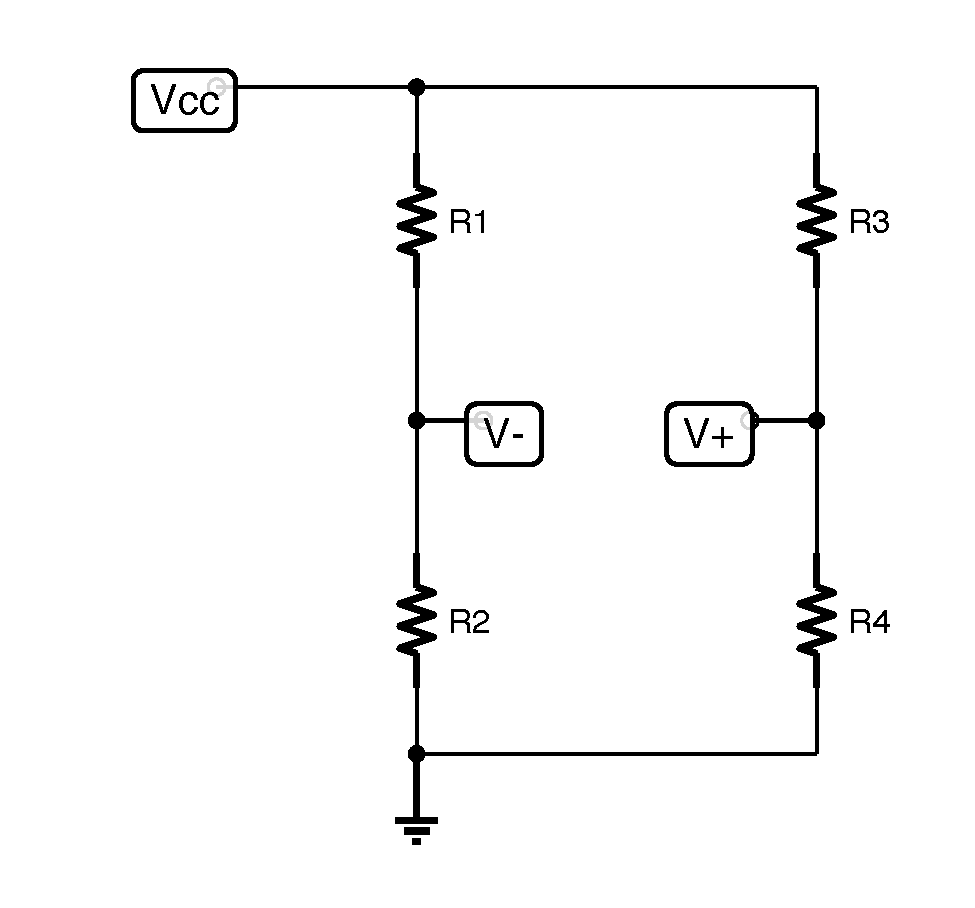
\includegraphics[width=\textwidth]{Wheatstone.pdf}
\caption{Esquemático elétrico de uma ponte de Wheatstone genérica.}
\label{fig:celula-comercial-circuito}
\end{figure}

\noindent onde os resistores $R_1$, $R_2$, $R_3$ e $R_4$ são valores de resistência elétrica que determinam o comportamento de ponte, $V_-$ e $V_+$ são os nós de saída da ponte medidos em tensão elétrica e $V_{cc}$ é a tensão elétrica de alimentação da ponte.

A função de transferência da ponte de Wheatstone proposta é dada conforme Equação \ref{eq:wheatstone-tf}:

\begin{equation}
	V_o = V_+ - V_- = \left(\dfrac{R_4}{R_4 + R_3} - \dfrac{R_2}{R_1 + R_2}\right)V_{cc}
	\label{eq:wheatstone-tf}
\end{equation}

Considerando que as condições da Equação \ref{eq:celula-comercial-cond1} ou \ref{eq:celula-comercial-cond2} são válidas, então a ponte é dita estar "em equilíbrio", isto é, a saída de tensão elétrica entre $V_-$ e $V_+$ é de $0V$.

\begin{eqnarray}
	R_1 R_4 = R_2 R_3 \label{eq:celula-comercial-cond1} \\
	R_1/R_3 = R_2/R_4 \label{eq:celula-comercial-cond2}
\end{eqnarray} 

Qualquer pequena variação de resistência elétrica em qualquer um dos resistores da Figura \ref{fig:celula-comercial-circuito} que violem as condições da Equação \ref{eq:celula-comercial-cond1} ou \ref{eq:celula-comercial-cond2} incorre no desequilíbrio da ponte, que pode ser medido utilizando a saída em tensão elétrica.

Com isto, a ponte pode ser utilizada como circuito de condicionamento para um sistema de medição de deformação mecânica de um corpo. Como já verificado, um extensômetro ou \textit{strain gage} (SG) é um resistor com um valor fixo ($R_0$) mais um valor variável ($\Delta R$) devido à deformação percebida. Utilizando $R_1=R_2=R_3=R_4$, e ainda com $r=R_2/R_1$, a variação de tensão na saída da ponte fica:

\begin{equation}
	\Delta E=\frac{V r}{(r+1)^2}\left [ \frac{\Delta R_1}{R_1}-\frac{\Delta R_2}{R_2}-\frac{\Delta R_3}{R_3}+\frac{\Delta R_4}{R_4} \right ]
	\label{eq:wheatstone-deltaE}
\end{equation}

É comum utilizar 3 formas distintas de medição utilizando extesômetros e a ponte de Wheatstone, que são vistas a seguir, usando como exemplo uma viga engastada.

\subsection{1/4 Ponte}

Nesta configuração, a mais simples delas, é utilizado apenas um strain gage (SG) ativo, conforme a Figura \ref{fig:1-4 ponte}. Os outros três são apenas resistores.

\begin{figure}[H]
\center
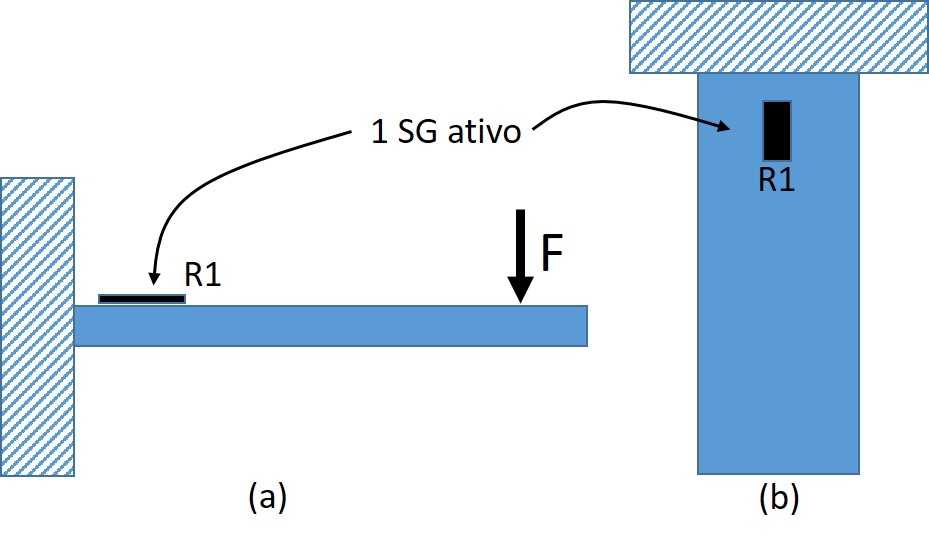
\includegraphics[width=0.7\textwidth]{1-4 ponte.jpg}
\caption{Modelo de fixação de SG para configuração de 1/4 Ponte. (a) vista lateral e (b) vista superior}
\label{fig:1-4 ponte}
\end{figure}

\noindent onde $R1$ representa a posição do SG e $F$ representa o ponto e sentido de aplicação da força.

Utilizando a Equação \ref{eq:wheatstone-deltaE}, com $\Delta R_{2,3,4}=0$ e $r=R_2/R_1=1$, tem-se:

\begin{equation}
	\Delta E=\frac{V r}{(r+1)^2}\left [ \frac{\Delta R_1}{R_1} \right ]=\frac{\Delta R}{4R}.V
	\label{eq:wheatstone-deltaE-1_4ponte}
\end{equation}

\subsection{1/2 Ponte}

Para a configuração de 1/2 Ponte são utilizados 2 SGs ativos, conforme verifica-se nas Figuras \ref{fig:1-2 ponte_sem temp} e \ref{fig:1-2 ponte_com temp}. A primeira delas, por apresentar os 2 SGs no mesmo lado da viga, isto é, sofrendo o mesmo tipo de deformação (alongamento), não permite a compensação dos efeitos de temperatura. Já o segundo exemplo consegue fazer a compesação, com os 2 SGs na mesma posição, mas em lados opostos da viga, pois um SG é alongando e outro comprimindo.

\begin{figure}[H]
\center
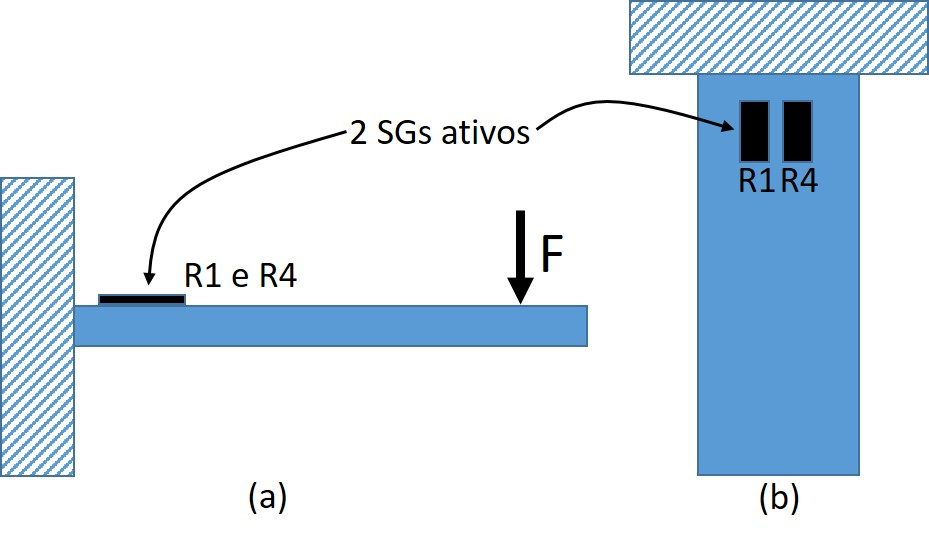
\includegraphics[width=0.7\textwidth]{1-2 ponte_1.jpg}
\caption{Modelo de fixação de SG para configuração de 1/2 Ponte sem compensação de temperatura. (a) vista lateral e (b) vista superior}
\label{fig:1-2 ponte_sem temp}
\end{figure}

\begin{figure}[H]
\center
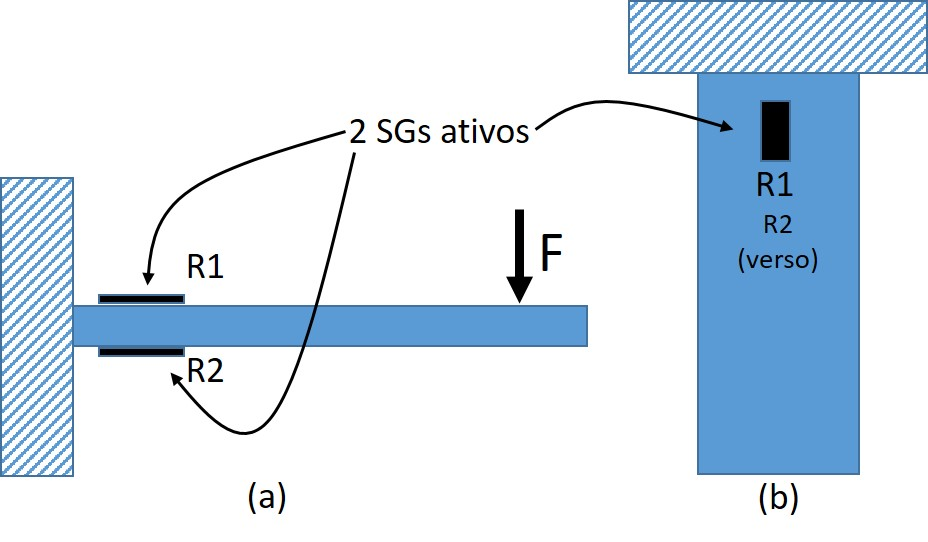
\includegraphics[width=0.7\textwidth]{1-2 ponte_2.jpg}
\caption{Modelo de fixação de SG para configuração de 1/2 Ponte com compensação de temperatura. (a) vista lateral e (b) vista superior}
\label{fig:1-2 ponte_com temp}
\end{figure}

\noindent onde $R_1$, $R_2$ e $R_4$ representam as posições dos SGs e $F$ representa o ponto e sentido de aplicação da força.

Analisando-se a aplicação da Equação \ref{eq:wheatstone-deltaE} para as duas situações apresentadas, tem-se

\begin{equation}
	\Delta E=\frac{V r}{(r+1)^2}\left [ \frac{\Delta R_1}{R_1}+\frac{\Delta R_4}{R_4} \right ]=\frac{\Delta R}{2R}.V
	\label{eq:wheatstone-deltaE-1_2ponte_sem_comp}
\end{equation}

\begin{equation}
	\Delta E=\frac{V r}{(r+1)^2}\left [ \frac{\Delta R_1}{R_1}-\frac{\Delta R_2}{R_2} \right ]=\frac{\Delta R}{2R}.V
	\label{eq:wheatstone-deltaE-1_2ponte_com_comp}
\end{equation}

Aparentemente, as duas equações resultam em um mesmo resultado, já que a deformação de $R_2$ é negativa, a menos que se perceba que:

\begin{equation}
	\frac{\Delta R_i}{R_i}=\frac{\Delta R_{\varepsilon_i}}{R_i}+\frac{\Delta R_{T_i}}{R_i}
	\label{eq:compensacao-temp}
\end{equation}

\noindent isto é, a variação do SG refere-se uma parte à deformação mecânica percebida ($\Delta R_{\varepsilon_i}$) e outra parte à variação de temperatura ($\Delta R_{T_i}$).

Assim, na configuração com compensação de temperatura, a variação de temperatura percebida por um dos SGs é anulada pela variação percebida pelo outro SG.

\subsection{Ponte Completla}

Esta configuração é a mais completa utilizando-se ponte de Wheatstone e SGs. A Figura \ref{fig:ponte-completa} exemplifica a posição dos SGs para a aplicação em uma viga engastada.

\begin{figure}[H]
\center
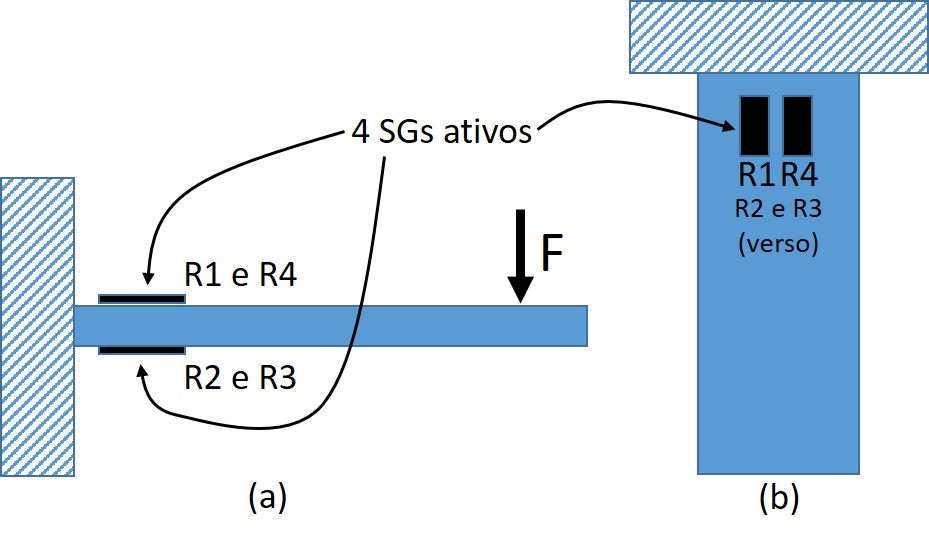
\includegraphics[width=0.7\textwidth]{ponte completa.jpg}
\caption{Modelo de fixação de SG para configuração de Ponte Completa. (a) vista lateral e (b) vista superior}
\label{fig:ponte-completa}
\end{figure}

\noindent onde $R_1$, $R_2$, $R_3$ e $R_4$ representam as posições dos SGs e $F$ representa o ponto e sentido de aplicação da força.

Nesta situação, onde $R_1$ e $R_4$ são fixados na parte superior da viga (alongando), e $R_2$ e $R_3$ são fixados nas mesmas posições, mas na parte inferior da viga (comprimindo), há a compensação do efeito da temperatura, e a Equação \ref{eq:wheatstone-deltaE-completa} apresenta a expressão da variação de tensão nos terminais da ponte.

\begin{equation}
	\Delta E=\frac{V r}{(r+1)^2}\left [ \frac{\Delta R_1}{R_1}-\frac{\Delta R_2}{R_2}-\frac{\Delta R_3}{R_3}+\frac{\Delta R_4}{R_4} \right ]=\frac{\Delta R}{R}.V
	\label{eq:wheatstone-deltaE-completa}
\end{equation}

Com certeza essa é o melhor dos 3 casos apresentados, haja vista que a sensibilidade da célula, conforme a Equação \ref{eq:wheatstone-sensibilidade-celula} , fica quatro vezes maior do que o caso de 1/4 ponte.

\begin{equation}
	S_c=\frac{\Delta E}{\varepsilon}
	\label{eq:wheatstone-sensibilidade-celula}
\end{equation}

\section{Célula de carga comercial}

Neste experimento foi levantada a função de transferência experimental para uma viga engastada utilizando uma célula de carga comercial "REACCION BCD-5" manufaturada por "FLEXAR Celdas de Carga".

Na Figura \ref{fig:celula-comercial-esquema-fisico} está apresentado um esquemático físico da célula de carga comercial utilizada:

\begin{figure}[H]
\center
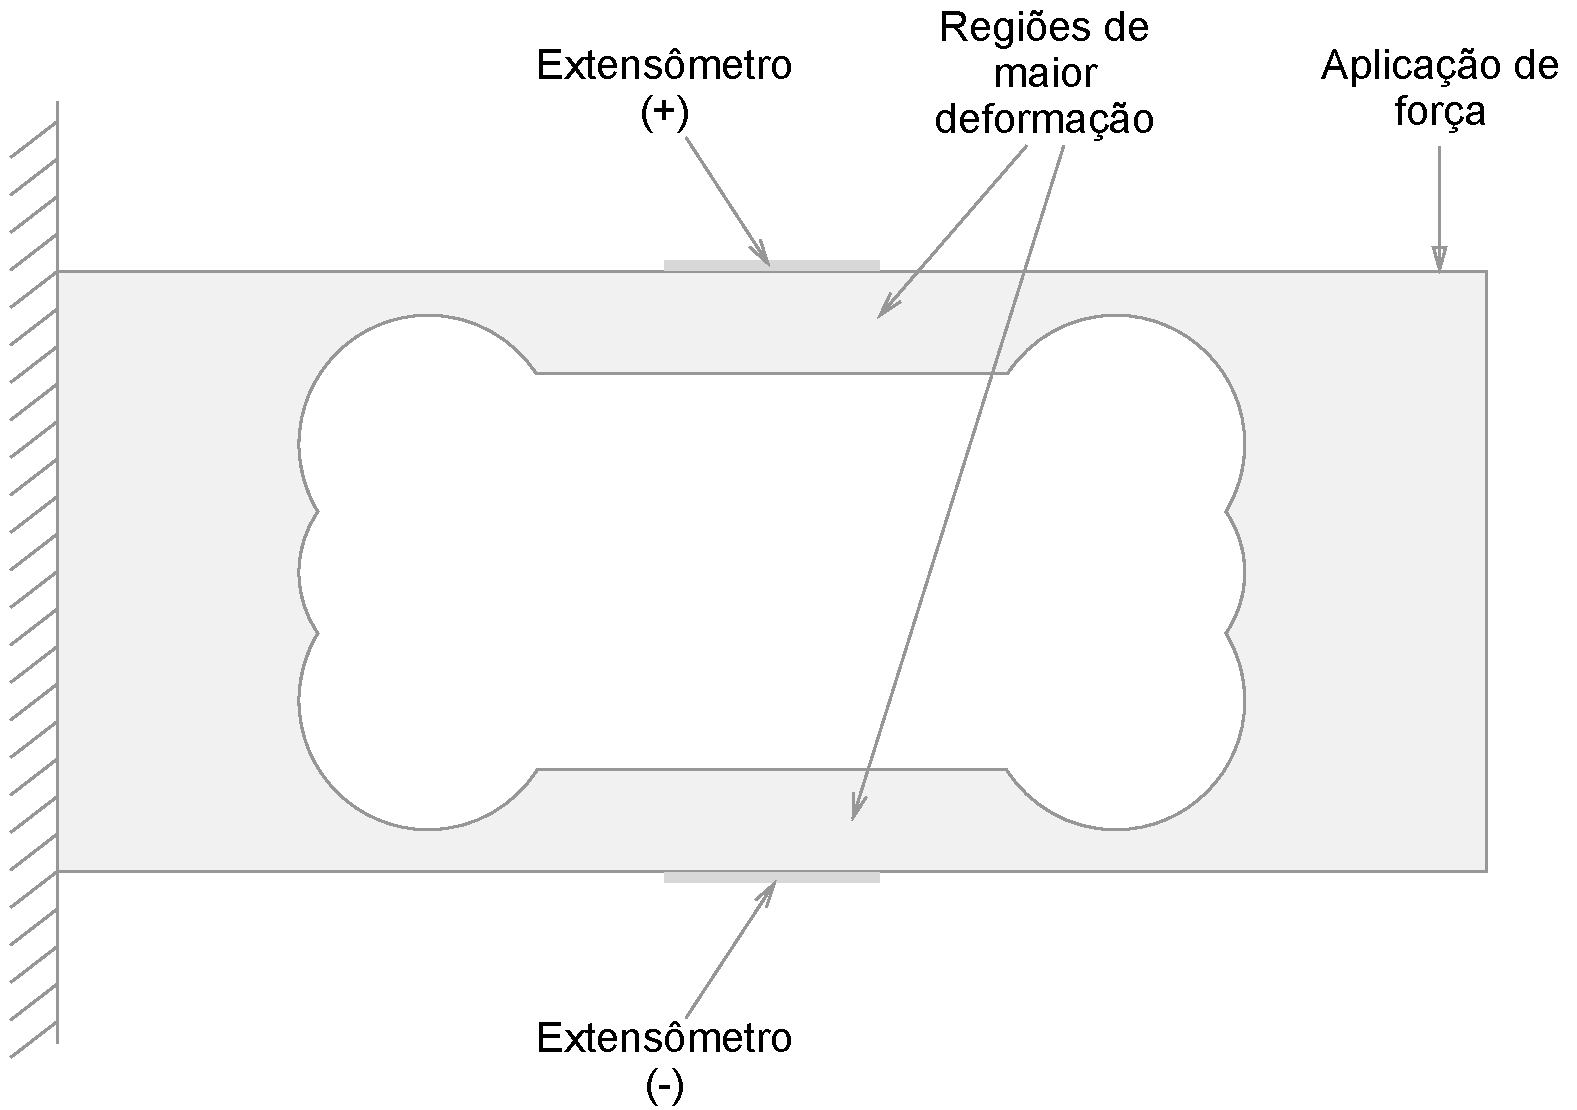
\includegraphics[width=\textwidth]{CelulaComercial.pdf}
\caption{Esquemático da construção mecânica da célula de carga comercial utilizada no experimento.}
\label{fig:celula-comercial-esquema-fisico}
\end{figure}

\noindent onde o extensômetro $(+)$ indica uma deformação positiva (alongamento) e o extensômetro $(-)$ indica uma deformação negativa (compressão).

Portanto, é possível utilizar esta construção como forma de medir deformações que a viga proposta esteja submetida.

De acordo com o fabricante a sensibilidade da célula é de $2 mV/V$ e possui $350 \Omega$ de resistência elétrica nominal e com carga máxima de $5 kg$.  O fabricante da célula é "FLEXAR Celdas de Carga", um fabricante argentino de células de carga, modelo "REACCION BCD-5". O site do fabricante não possuía listagem com especificações técnicas deste modelo e portanto não há informações mais detalhadas sobre esta célula, como incertezas da resistência nominal, incerteza da sensibilidade e outros detalhes.

Todas medidas de tensão elétrica da célula foram feitas utilizando o LabVIEW versão 7.1 disponibilizada pelo laboratório com auxílio dos dispositivos de DAQ da National Instruments modelo USB-6009. Conforme o fabricante \cite{daq-specifications} a entrada analógica deste dispositivo possui 14 bits, taxa de amostragem de 48 kS/s e resolução de tensão elétrica de 1.53mV. O sinal de saída foi amostrado à uma taxa de 1000 Hz com 500 amostras e a média destes valores era tomado como uma única medida experimental. Este processo visa minimizar o impacto do ruído aditivo gaussiano branco (AWGN) gerado pelo circuito de condicionamento na medida realizada.

O circuito de condicionamento consistia em um amplificador de instrumentação (AI) INA126AP fabricado pela Texas Instruments com \textit{bias} de corrente de entrada máxima de 25 nA \cite{datasheet-ina126} configurado com ganho de 29.24 vezes. O circuito de condicionamento foi alimentado utilizando um regulador de tensão elétrica positivo LM7805 de $5V \pm 0,2V$ \cite{datasheet-lm7805} fabricado pela Fairchild Semiconductors e com um regulador de tensão elétrica negativo LM7905 de $-5V \pm 0,2V$ \cite{datasheet-lm7905} fabricado pela Texas Instruments. A célula de carga foi alimentada utilizando a referência de tensão elétrica REF02 de $5V \pm 0,01V$ \cite{datasheet-ref02} fabricado pela Texas Instruments.

A Figura \ref{fig:celula-comercial-metodologia-condicionamento} apresenta o esquemático elétrico do circuito de condicionamento da célula de carga.

\begin{figure}[H]
\center
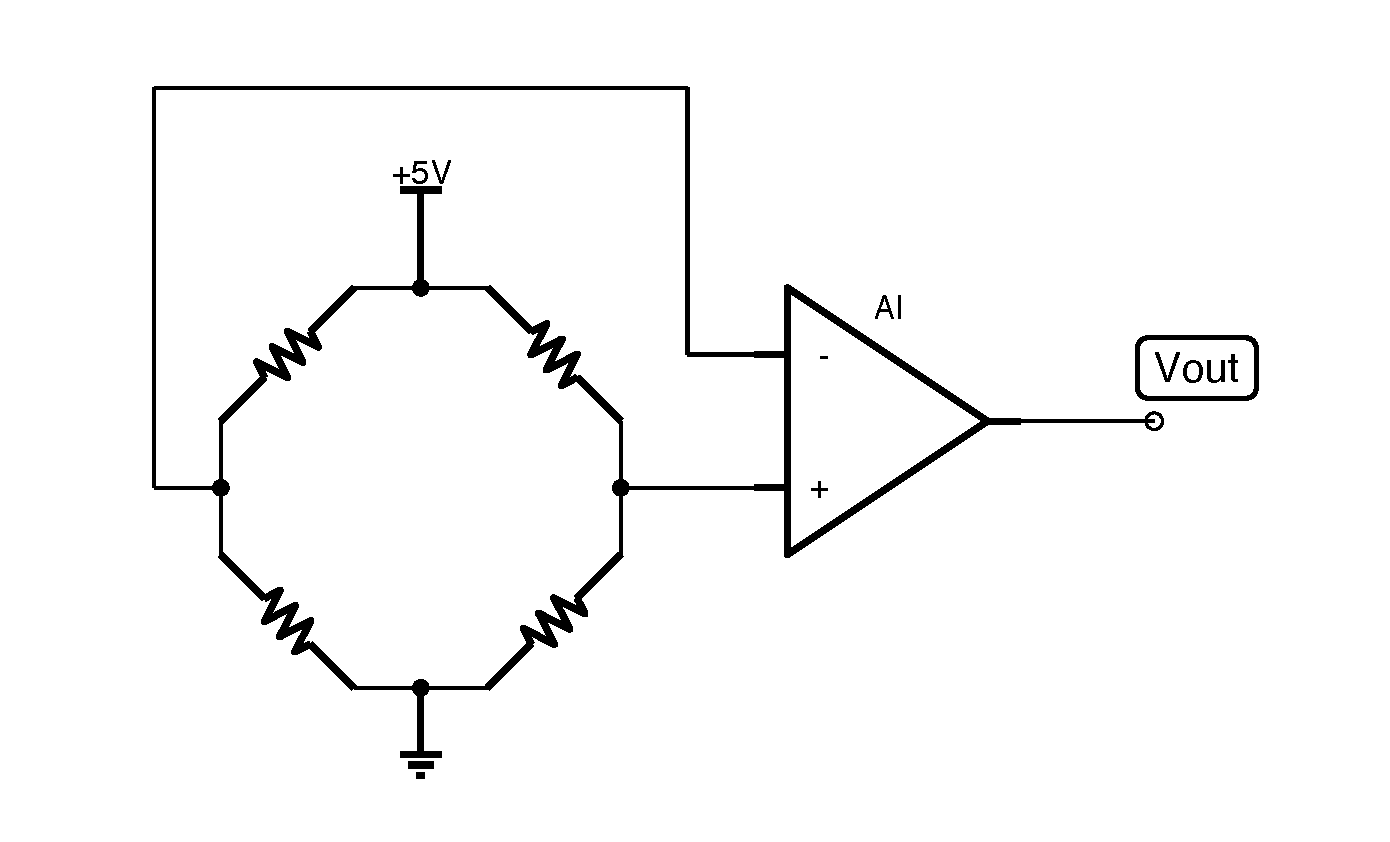
\includegraphics[width=\textwidth]{Comercial-Circuito.pdf}
\caption{Esquemático elétrico do circuito de condicionamento da célula de carga comercial}
\label{fig:celula-comercial-metodologia-condicionamento}
\end{figure}

\noindent onde a alimentação de $+5V$ representa a referência de tensão elétrica REF02, os resistores representam de forma simbólica a ponte de Wheatstone interna da célula de carga (o fabricante não informa de forma exata a topologia de construção da ponte nem valores de resistores que colaboram no balanço da ponte), o amplificador AI é um amplificador de instrumentação com ganho de 29.24 e $V_{out}$ é a tensão elétrica de saída da ponte, filtrado, amostrado pelo DAQ e medido no LabVIEW.

O circuito de amostragem consistia em um filtro passa-baixas de Butterworth de ordem 4 com frequência de corte de 100Hz utilizando a topologia de filtros analógicos ativos de Sallen-Key. Como amplificador operacional para a implementação do filtro, utilizou-se o amplificador operacional encapsulado TL084 da Texas Instruments com distorção harmônica total típica de $0,003\%$ \cite{datasheet-tl084}.

A Figura \ref{fig:celula-comercial-cadeia-transducao} apresenta a cadeia de transdução completa utilizada no experimento.

\begin{figure}[H]
\center
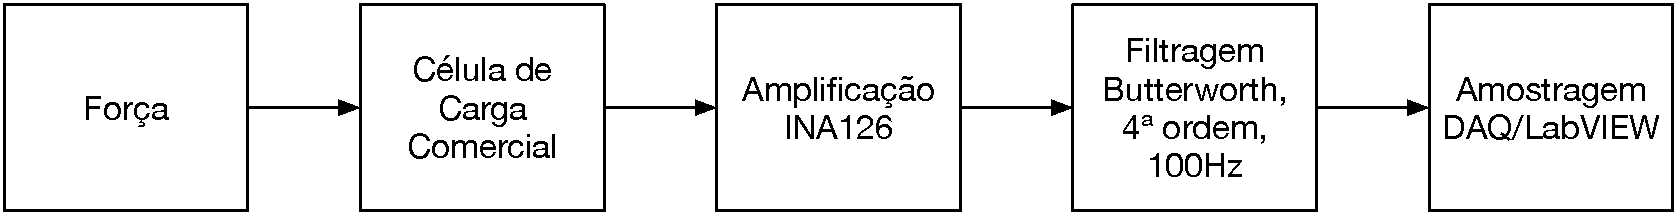
\includegraphics[width=\textwidth]{Comercial-Cadeia-Transducao.pdf}
\caption{Cadeia de transdução completa do experimento com a célula de carga comercial}
\label{fig:celula-comercial-cadeia-transducao}
\end{figure}

A Figura \ref{fig:celula-comercial-cadeia-medidas} mostra a cadeia de medidas proposta para o experimento utilizando a célula de carga comercial.

\begin{figure}[H]
\center
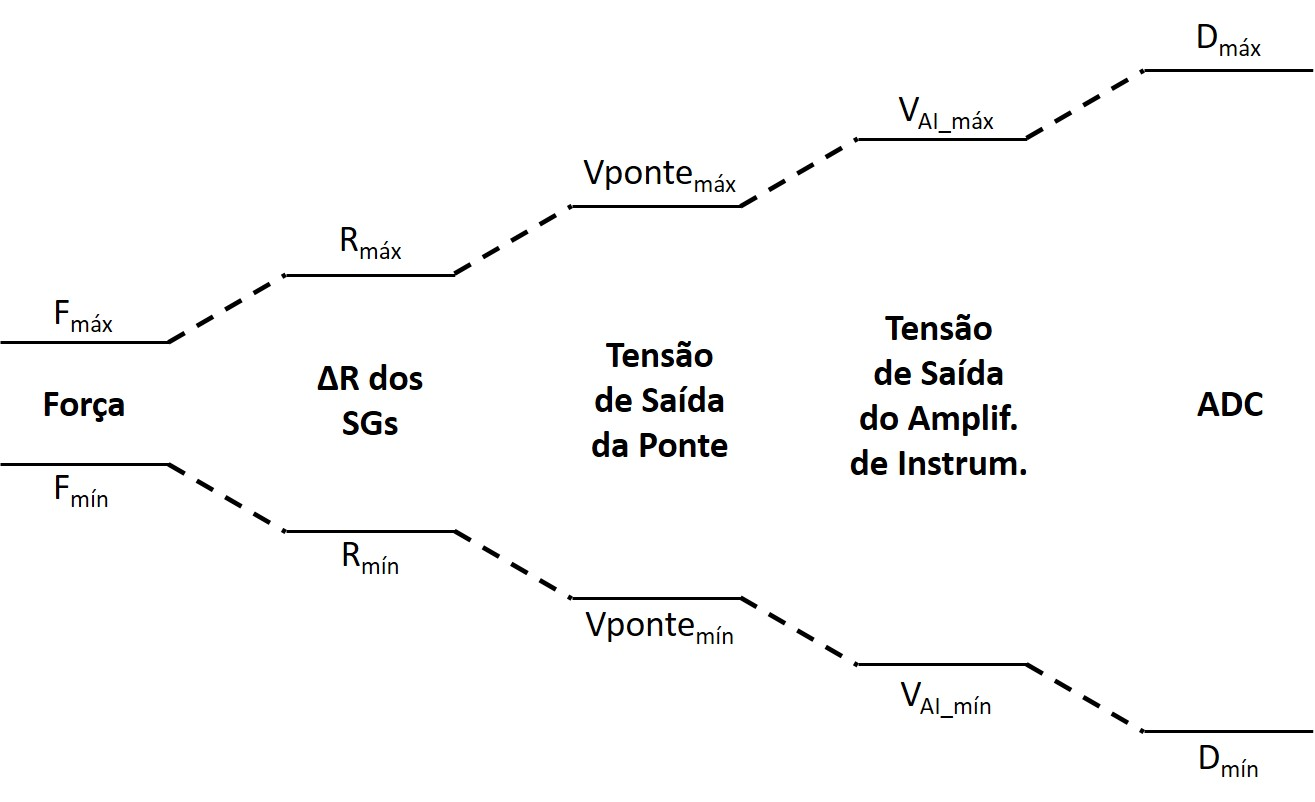
\includegraphics[width=0.7\textwidth]{CadeiaMedidasProposta_Celula.jpg}
\caption{Cadeia de medidas proposta para o experimento com a célula de carga comercial}
\label{fig:celula-comercial-cadeia-medidas}
\end{figure}


\section{Célula de carga não-comercial}

A célula de carga não comercial utilizada possuía a configuração dada na Figura \ref{fig:celula-nao-comercial-desenho}:

\begin{figure}[H]
\center
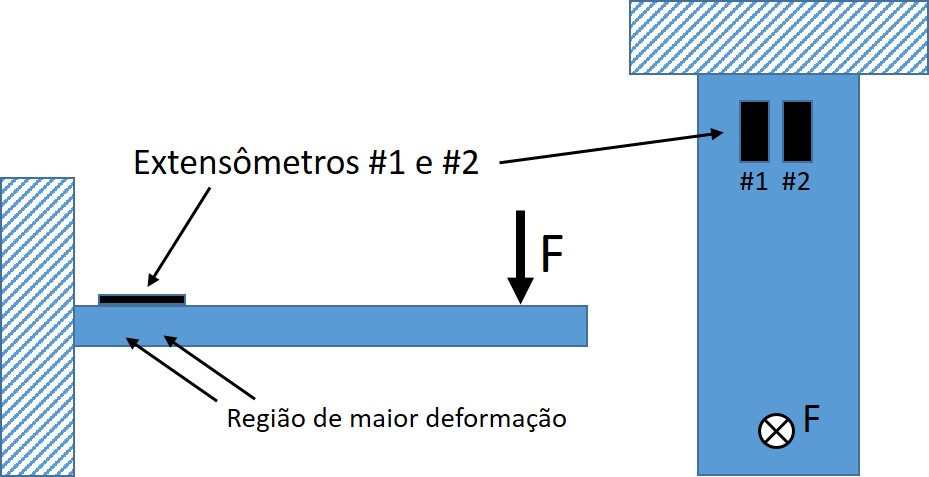
\includegraphics[width=0.7\textwidth]{CelulaNaoComercial_2.jpg}
\caption{Esquemático da construção mecânica da célula de carga não-comercial utilizada no experimento.}
\label{fig:celula-nao-comercial-desenho}
\end{figure}

\noindent onde os extensômetros $\#1$ e $\#2$ percebem uma deformação positiva (alongamento) e $F$ indica a posição e direção da força aplinada. É importante observar que, na verdade, a viga possuía 4 extensômetros (2 na parte superior e 2 na parte inferior), formando um sistema de ponte completa. Porém, havia indicativos de não funcionamento dos extensômetros da parte inferior, razão esta que fez com que se optasse pelo uso dos extensômetros da parte superior. Por estarem colocados lado-a-lado na viga, espera-se que suas deformações sejam idênticas.

Ao contrário da célula comercial, esta não possui a ponte pré-calibrada e, portanto, se fez necessário que a ponte fosse calibrada e ajustada para obter o resultado desejado. Como não havia especificação dos extensômetros (modelos e fabricantes não estavam explícitos sobre a construção) não foi possível comparar com os valores fornecidos pelo fabricante. Havia, contudo, uma marcação indicando o valor de resistência nominal do extensômetro.

Considerando que a resistência elétrica nominal da célula de carga quando em repouso seja de $350 \Omega$ com incerteza desconhecida, é possível calcular os resistores para os demais braços da ponte de Wheatstone. A Figura \ref{fig:celula-nao-comercial-ponte}

\begin{figure}[H]
\center
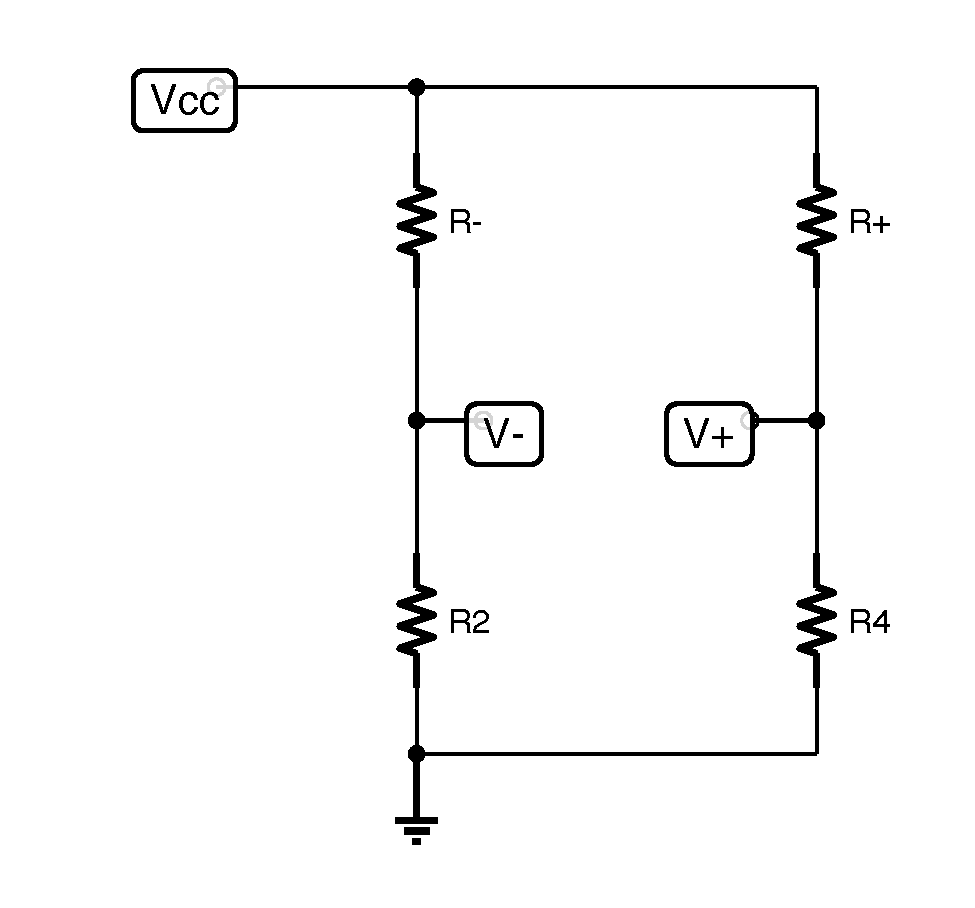
\includegraphics[width=0.7\textwidth]{WheatstoneNaoComercial.pdf}
\caption{Esquemático elétrico da ponte de Wheatstone para a célula de carga não-comercial. O modelo escolhido foi utilizar uma meia-ponte, com ambos SGs com variação positiva.}
\label{fig:celula-nao-comercial-ponte}
\end{figure}

\noindent onde os resistores $R_1$ e $R_2$ são resistores cujo valor deve ser o mais próximo possível do valor nominal dos extensômetros da ponte e $R+_1$ e $R+_2$ são os extensômetros localizados na parte superior da viga ,com variação positiva de resistência elétrica em função da deformação da barra.

Todas medidas de tensão elétrica da célula foram feitas utilizando o LabVIEW versão 7.1 disponibilizada pelo laboratório com auxílio dos dispositivos de DAQ da National Instruments modelo USB-6009. Conforme o fabricante \cite{daq-specifications} a entrada analógica deste dispositivo possui 14 bits, taxa de amostragem de 48 kS/s e resolução de tensão elétrica de 1.53mV. O sinal de saída foi amostrado à uma taxa de 1000 Hz com 500 amostras e a média destes valores era tomado como uma única medida experimental. Este processo visa minimizar o impacto do ruído aditivo gaussiano branco (AWGN) gerado pelo circuito de condicionamento na medida realizada.

O circuito de condicionamento consistia em um amplificador de instrumentação (AI) INA126AP fabricado pela Texas Instruments com \textit{bias} de corrente de entrada máxima de 25 nA \cite{datasheet-ina126} configurado com ganho de 29.24. O circuito de condicionamento foi alimentado utilizando um regulador de tensão elétrica positivo LM7805 de $5V \pm 0,2V$ \cite{datasheet-lm7805} fabricado pela Fairchild Semiconductors e com um regulador de tensão elétrica negativo LM7905 de $-5V \pm 0,2V$ \cite{datasheet-lm7905} fabricado pela Texas Instruments. A ponte de Wheatstone da célula de carga foi alimentada utilizando a referência de tensão elétrica REF02 de $5V \pm 0,01V$ \cite{datasheet-ref02} fabricado pela Texas Instruments.

%A Figura \ref{fig:celula-nao-comercial-metodologia-condicionamento} apresenta o esquemático elétrico do circuito de condicionamento da célula de carga.
%
%\begin{figure}[H]
%\center
%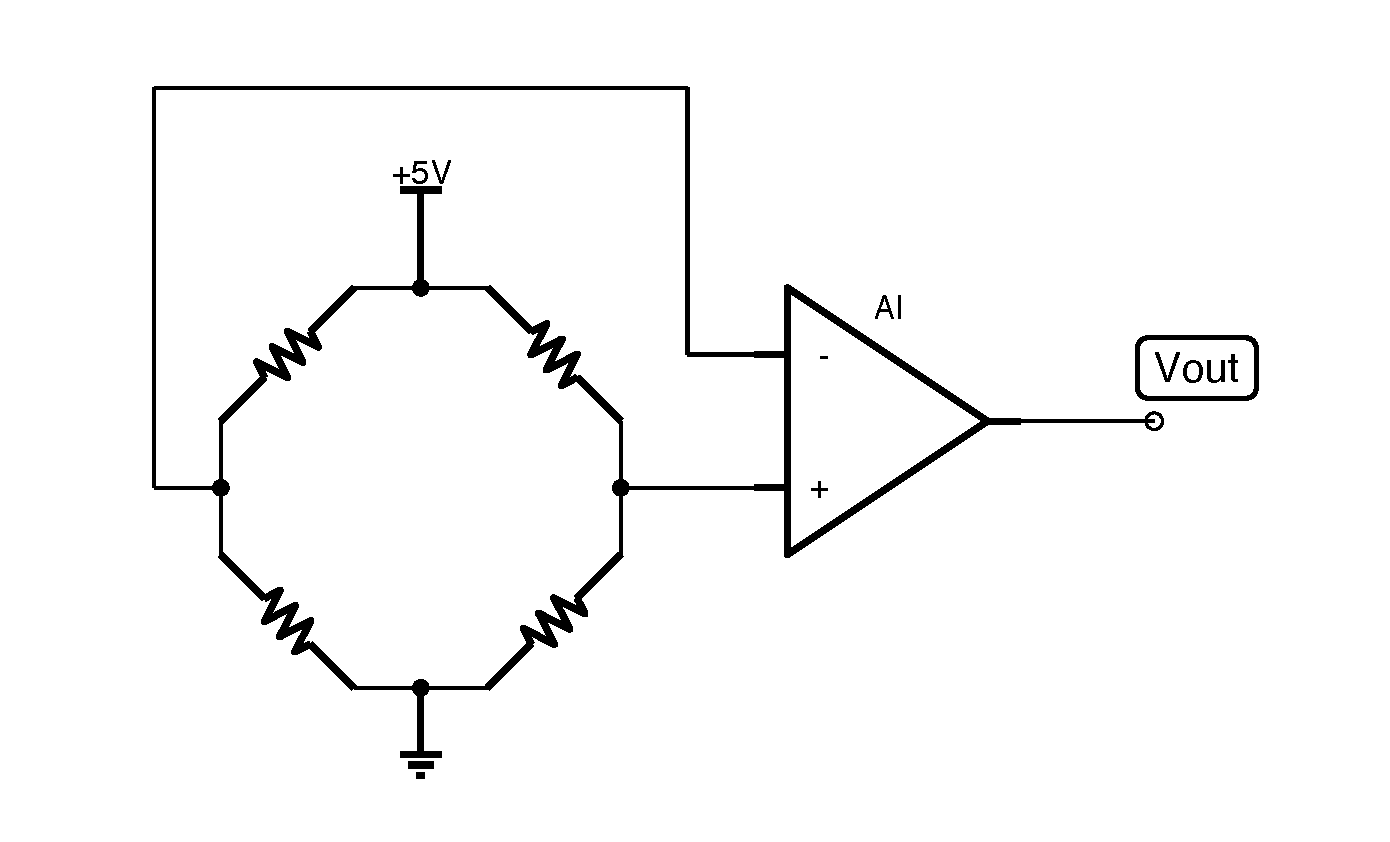
\includegraphics[width=\textwidth]{Comercial-Circuito.pdf}
%\caption{Esquemático elétrico do circuito de condicionamento da célula de carga comercial}
%\label{fig:celula-nao-comercial-metodologia-condicionamento}
%\end{figure}
%
%\noindent onde a alimentação de $+5V$ representa a referência de tensão elétrica REF02, os resistores representam de forma simbólica a ponte de Wheatstone interna da célula de carga (o fabricante não informa de forma exata a topologia de construção da ponte nem valores de resistores que colaboram no balanço da ponte), o amplificador AI é um amplificador de instrumentação com ganho de \todo{quanto?} e $V_{out}$ é a tensão elétrica de saída da ponte, filtrado, amostrado pelo DAQ e medido no LabVIEW.
%
O circuito de amostragem consistia em um filtro passa-baixas de Butterworth de ordem 4 com frequência de corte de 100Hz utilizando a topologia de filtros analógicos ativos de Sallen-Key. Como amplificador operacional para a implementação do filtro, utilizou-se o amplificador operacional encapsulado TL084 da Texas Instruments com distorção harmônica total típica de $0,003\%$ \cite{datasheet-tl084}.

A Figura \ref{fig:celula-nao-comercial-cadeia-transducao} apresenta a cadeia de transdução completa utilizada no experimento.

\begin{figure}[H]
\center
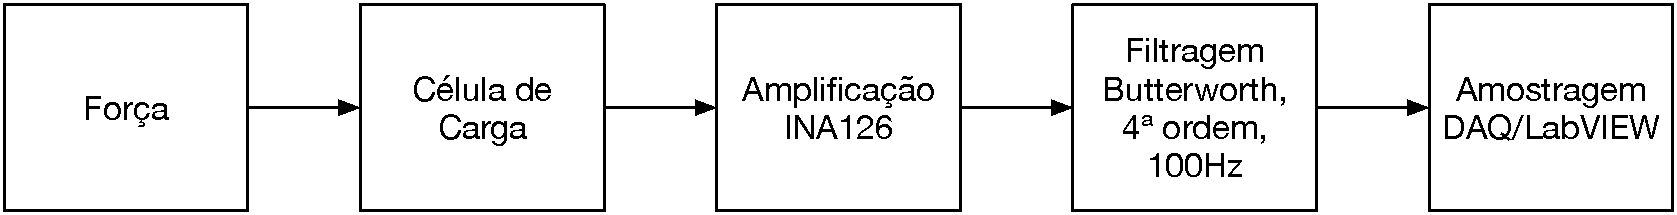
\includegraphics[width=\textwidth]{NaoComercial-Cadeia-Transducao.pdf}
\caption{Cadeia de transdução completa do experimento com a célula de carga não-comercial}
\label{fig:celula-nao-comercial-cadeia-transducao}
\end{figure}

A Figura \ref{fig:celula-nao-comercial-cadeia-medidas} mostra a cadeia de medidas proposta para o experimento utilizando a célula de carga não comercial.

\begin{figure}[H]
\center
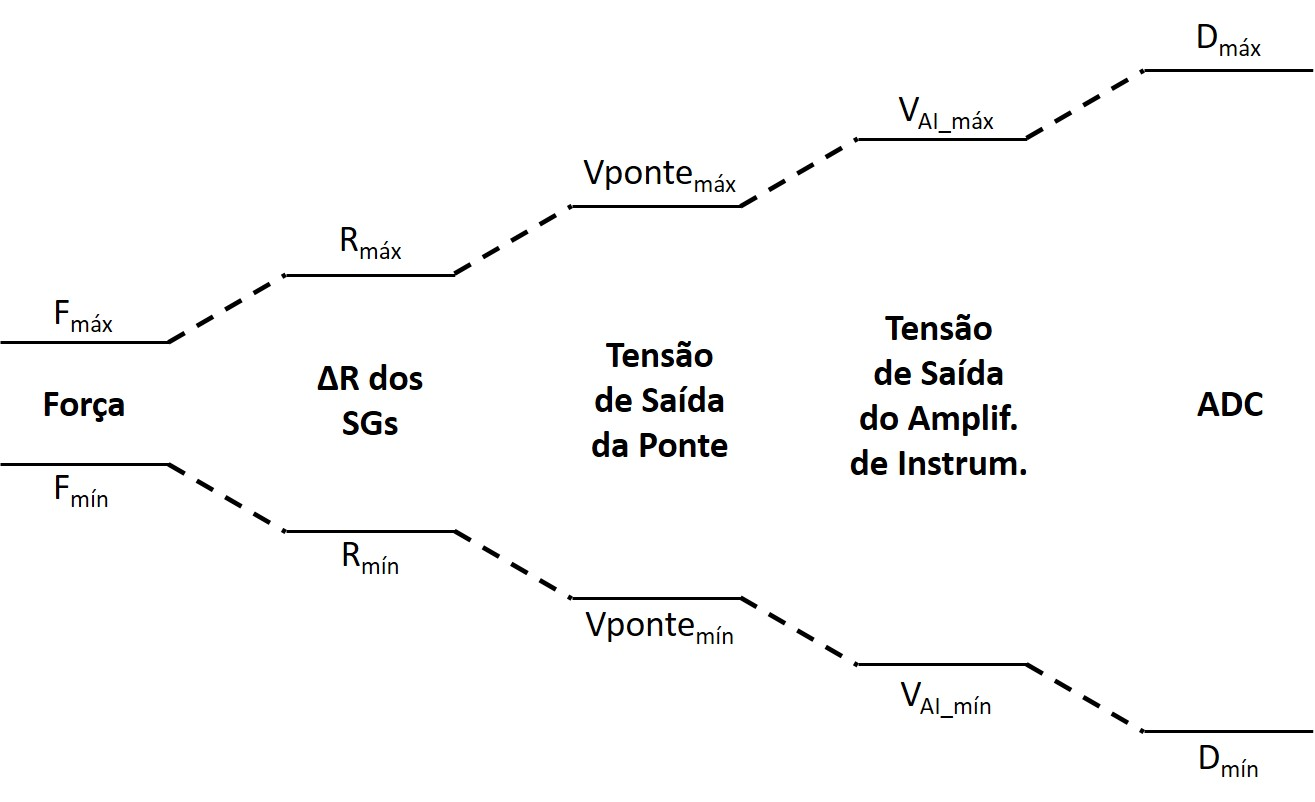
\includegraphics[width=0.7\textwidth]{CadeiaMedidasProposta_Celula.jpg}
\caption{Cadeia de medidas proposta para o experimento com a célula de carga não comercial}
\label{fig:celula-nao-comercial-cadeia-medidas}
\end{figure}

Para estimar a frequência natural de ressonância do sistema, um experimento de aquisição de dados temporalmente foi projetado. Neste experimento a barra foi batida com uma ferramenta de metal e sem carga. O curva temporal de resposta da barra foi adquirida e armazenada num arquivo TSV (\textit{tab separated values}), após, utilizando softwares de processamento matemático, foi extraída a transformada de Fourier deste sinal.

A transformada de Fourier do sinal deve possuir picos de magnitude na frequência natural de vibração da célula. Isto se deve ao fato da barra ter uma tendência a vibrar em algumas frequências específicas e amortecer outras frequências não-harmônicas desta fundamental. Este resultado é importante, pois caso a viga esteja próxima de alguma fonte capaz de produzir vibrações nesta frequência a célula pode entrar em ressonância e quebrar ou ter danos estruturais.

Outra análise importante a ser feita com sensores resistivos é de resposta térmica. Saber se um sistema de medida tem variação da temperatura e como ele varia com a temperatura é fundamental. Um sistema ideal é invariante em função da temperatura, isto é, independente da temperatura sua resposta é sempre igual. Na realidade, isto é muito difícil de acontecer, resistências elétricas variam com a temperatura e sistemas mecânicos deformam e dilatam com a variação de temperatura.

Uma das vantagens do uso de ponte de Wheatstone completa ou 1/2 ponte, com sensores em lados inversos da viga, é que é a forma mais robusta em função da variação de temperatura, a variação de resistência dos extensômetros devido à variação térmica é mínima e considerando que o aquecimento se dê de forma uniforme nos 4 sensores, o efeito de aquecimento é anulado pela própria ponte de Wheatstone.

Neste experimento a fim de determinar o comportamento do sistema quando aquecido foi aquecido a face inferior da célula (longe dos extensômetros) durante 4 minutos. Estes dados foram adquiridos e filtrados digitalmente para remover o ruído gerado pelo circuito de condicionamento e conversor analógico-digital da placa de aquisição de dados. Neste tipo de experimento, mesmo em se tratando dos modelos que compensam os efeitos térmicos, é praticamente impossível, sob as condições existentes, garantir que a barra tenha aquecimento homogêneo e, portanto, provoque a mesma variação de resistência elétrica correlacionada com o aumento de temperatura. 

O processo de aquisição de dados para a análise de frequência fundamental como a análise de comportamento térmico foi utilizado o mesmo processo de calibração do sistema.

\subsection{Modelo computacional}
A fim de realizar uma validação computacional dos resultados, foi desenvolvido um modelo computacional para a célula de carga não-comercial no software SOLIDWORKS 2016 x64 e realizada utilizando o método FFEPlus com a opção de \textit{large displacement} desativada.

Na simulação de análise estática da célula, foi aplicada uma força de 4N sobre o furo presente na barra. A Figura \ref{fig:celula-nao-comercial-solid-modelo} apresenta o modelo 3D desenvolvido no software:

\begin{figure}[H]
\center
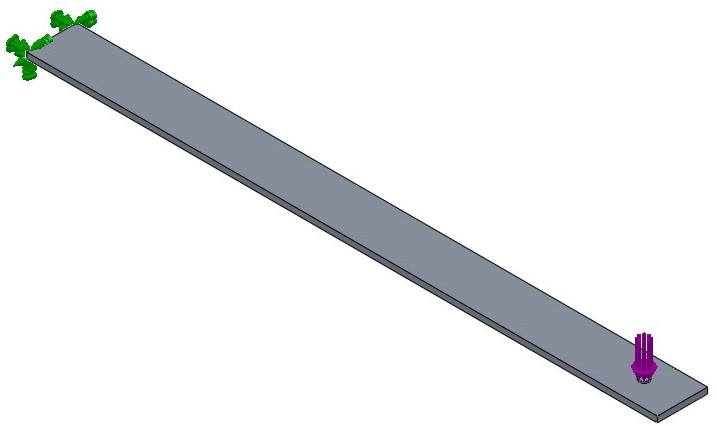
\includegraphics[width=0.7\textwidth]{CelulaNaoComercial_solid.jpg}
\caption{Modelo 3D utilizado para a simulação da célula de carga não-comercial no SOLIDWORKS.}
\label{fig:celula-nao-comercial-solid-modelo}
\end{figure}

\noindent onde a superfície de aplicação da força é o orifício utilizado para exercer as forças durante a execução do experimento no laboratório.

Nesta simulação foi possível estimar a deformação da barra para os valores de 2N, 4N, 6N, 8N e 10N que correspondem, aproximadamente aos pesos das massas de 200g, 400g, 600g, 800g e 1kg (considerando que a aceleração local da gravidade $g$ é dada, aproximadamente, por $10 m/s^2$.

A fim de determinar a frequência fundamental da vibração do sistema, foi realizada uma simulação dinâmica de frequência do sistema. Nesta simulação a frequência fundamental de vibração do sistema foi extraída e validada com o experimento em que uma batida é feita na barra e pela vibração medida pelo extensômetro é possível estimar a frequência fundamental de vibração do sistema.


\section{Torquímetro}
Neste experimento foi utilizado um torquímetro GEDORE FLEX-O-TORK Nº 4657 cujo ponto de maior torque (no eixo do torquímetro) haviam 4 extensômetros cimentados nos 4 lados do metal do cabo, portanto uma ponte completa. Com este sistema, é possível medir o toque exercido pelo operador no instrumento.

O torquímetro já estava construído e possuía 4 fios: 2 de alimentação (terra e alimentação positiva) e outros 2 fios para a saída: positivo e negativo. O sistema foi alimentado utilizando a referência de tensão elétrica REF02 de $5V \pm 0,01V$ \cite{datasheet-ref02} fabricado pela Texas Instruments, e o resultado foi observado com o multímetro Minipa, modelo ET-2082b, com as especificações de precisão informadas pelo fabricante apresentada na Tabela \ref{tab:precisão-multimetro}. A coluna da precisão é apresentada na forma: $\pm$ (a$\%$ leitura + b dígitos), garantido por 1 ano. Como equipamento já tem mais de um ano de uso sem calibragem, esses dados não são totalmente fidedígnos. Foi utilizada a faixa de $200 mV$.

\begin{table}[H]
\centering
\caption{Especificações de precisão do multímetro Minipa ET-2082B para a medição de Tensão DC}
\label{tab:precisão-multimetro}
\begin{tabular}{|c|c|c|}
\hline
\textbf{Faixa} & \textbf{Precisão} & \textbf{Resolução} \\ \hline
200 mV         & \multirow{4}{*}{$\pm$ (0.5\% + 3D)} & 100 $\mu$V \\ \cline{1-1} \cline{3-3} 
2 V            &                              & 1 mV               \\ \cline{1-1} \cline{3-3} 
20 V           &                              & 10 mV              \\ \cline{1-1} \cline{3-3} 
200 V          &                              & 100 mV             \\ \hline
1000 V         & $\pm$ (1.0\% + 5D)           & 1 V                \\ \hline
\end{tabular}
\end{table}

Para extrair a função de transferência experimental do torquímetro foi aplicado torque utilizando o medidor físico gravado sobre o instrumento na faixa de 0 a 60$lbf.ft$ (\textit{pound-force foot}).

A Figura \ref{fig:torquimetro-cadeia-medidas} mostra a cadeia de medidas proposta para o experimento utilizando o torquímetro.

\begin{figure}[H]
\center
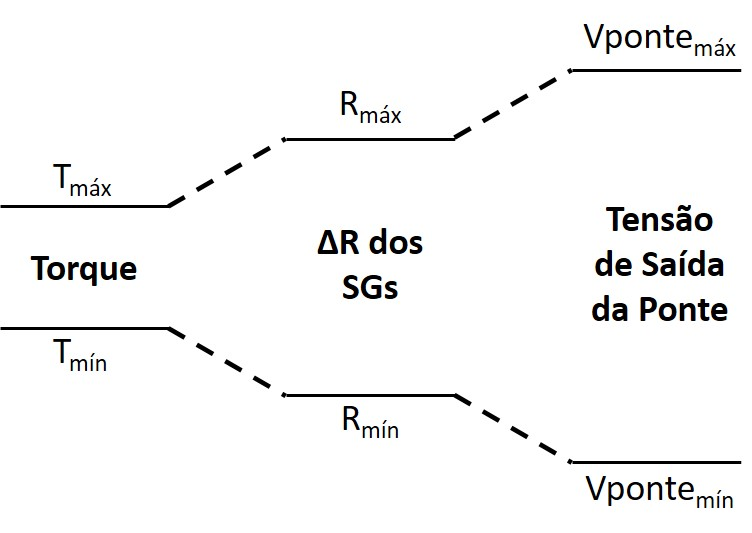
\includegraphics[width=0.7\textwidth]{CadeiaMedidasProposta_Torquimetro.jpg}
\caption{Cadeia de medidas proposta para o experimento com o torquímetro}
\label{fig:torquimetro-cadeia-medidas}
\end{figure}

\chapter{Resultados e Discussões}

\section{Célula de carga comercial}
A Tabela \ref{tab:celula-comercial-resultado-funcao-transferencia} apresenta as medidas experimentais para a célula de carga comercial.


\begin{table}[H]
\centering
\caption{Tabela com os valores medidos experimentalmente para ajuste da função de transferência experimental da célula de carga comercial.}
\begin{tabular}{|l|l|l|}

\hline
\textbf{Massa (kg)} & \textbf{Medida \#1 (V)} & \textbf{Medida \#2 (V)} \\ \hline
0.0 & 1.899 & 1.896 \\ \hline
0.2 & 1.887 & 1.885 \\ \hline
0.4 & 1.875 & 1.867 \\ \hline
0.6 & 1.863 & 1.858 \\ \hline
0.8 & 1.852 & 1.846 \\ \hline
1.0 & 1.841 & 1.834 \\ \hline
1.2 & 1.823 & 1.827 \\ \hline
1.4 & 1.818 & 1.811 \\ \hline
1.6 & 1.806 & 1.799 \\ \hline
1.8 & 1.795 & 1.788 \\ \hline
2.0 & 1.784 & 1.781 \\ \hline
2.2 & 1.766 & 1.769 \\ \hline
2.4 & 1.760 & 1.757 \\ \hline
2.6 & 1.748 & 1.743 \\ \hline
2.8 & 1.737 & 1.734 \\ \hline
3.0 & 1.724 & 1.718 \\ \hline
3.2 & 1.708 & 1.712 \\ \hline
3.4 & 1.702 & 1.695 \\ \hline
3.6 & 1.691 & 1.684 \\ \hline
3.8 & 1.679 & 1.671 \\ \hline
4.0 & 1.668 & 1.665 \\ \hline
4.2 & 1.652 & 1.654 \\ \hline
4.4 & 1.644 & 1.642 \\ \hline
4.6 & 1.631 & 1.631 \\ \hline
4.8 & 1.621 & 1.619 \\ \hline
5.0 & 1.609 & 1.608 \\ \hline

\end{tabular}
\label{tab:celula-comercial-resultado-funcao-transferencia}
\end{table}

A função que melhor ajusta os dados da Tabela \ref{tab:celula-comercial-resultado-funcao-transferencia} é dada na Equação \ref{eq:celula-comercial-resultado-funcao-transferencia}

\begin{equation}
	m(V) = 32.9198 - 17.3681 V
	\label{eq:celula-comercial-resultado-funcao-transferencia}
\end{equation}

\noindent onde $m(V)$ é a massa em $kg$ a qual a viga está submetida e $V$ é a tensão elétrica em $volts$ medida na saída da ponte de Wheatstone com o sensor.

A função foi ajustada com $R^2$ dado pela Equação \ref{eq:celula-comercial-resultado-funcao-transferencia-r2}. Já o erro de linearidade $\varepsilon_{L\%}$ encontrado devido à regressão foi de $3.09\%$.

\begin{equation}
	R^2 = 0.998975
	\label{eq:celula-comercial-resultado-funcao-transferencia-r2}
\end{equation}

A sensibilidade observada experimentalmente para a célula de carga comercial pode ser dada pela derivada da função de transferência experimental em razão da tensão elétrica, conforme a Equação \ref{eq:celula-comercial-sensibilidade-experimental}

\begin{equation}
	S_{experimental}=\frac{d (m(V))}{d V }=-17.368\frac{Kg}{V} \textrm{ ou } S_{experimental}=-57.6\frac{mV}{Kg}
	\label{eq:celula-comercial-sensibilidade-experimental}
\end{equation}


A Figura \ref{fig:celula-comercial-resultado-funcao-transferencia} apresenta um gráfico com a função de transferência da Equação \ref{eq:celula-comercial-resultado-funcao-transferencia} e os dados da Tabela \ref{tab:celula-comercial-resultado-funcao-transferencia}.

\begin{figure}[H]
\center
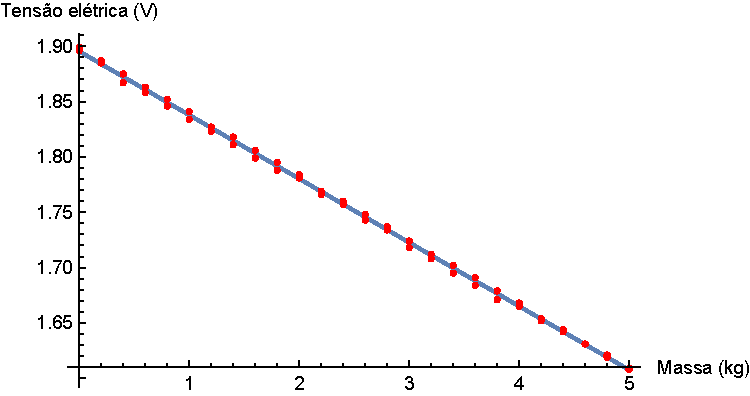
\includegraphics[width=\textwidth]{Comercial-Plot.pdf}
\caption{Função de transferência experimental: função de melhor ajuste e medidas experimentais}
\label{fig:celula-comercial-resultado-funcao-transferencia}
\end{figure}

\noindent onde a linha contínua representa a função ajustada e os pontos representam cada medida individual realizada.

Na Figura \ref{fig:celula-comercial-cadeia-medidas-experimental} pode-se verificar a cadeia de medidas experimental que foi executada para a célula de carga comercial. Nota-se que não foi possível adquirir os valores de resistência elétrica dos extensômetros, haja vista se tratar de uma estrutura fechada, sem acesso a cada um dos sensores, estando disponível apenas os terminais da ponte interna.

\begin{figure}[H]
\center
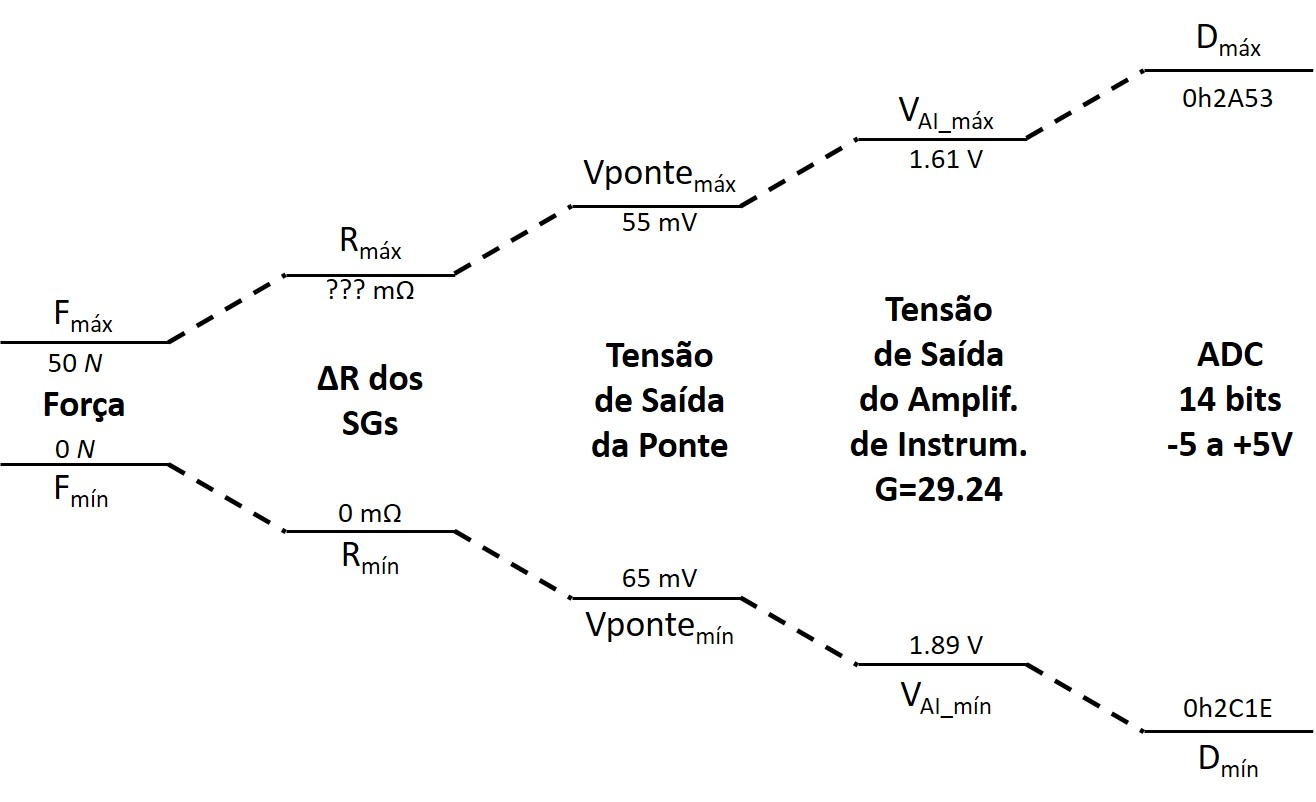
\includegraphics[width=0.7\textwidth]{CadeiaMedidasExperimental_CelulaComercial.jpg}
\caption{Cadeia de medidas experimental executada para a célula de carga comercial}
\label{fig:celula-comercial-cadeia-medidas-experimental}
\end{figure}


Com a função de transferência é possível aplicá-la nos dados adquiridos em laboratórios e obter a resposta da célula para a adição ou remoção de carga.

A Figura \ref{fig:celula-comercial-resultado-0-1kg} apresenta a resposta da célula quando adicionado uma massa suspensa de $1 kg$ na barra. Uma força equivalente de aproximadamente 10N é exercida sobre a barra (assumindo que a aceleração da gravidade local $g$ seja de $10 m/s^2$). A curva foi filtrada por um filtro passa-baixas digital com frequência de corte de 5Hz para reduzir o efeito do ruído gerado pelo circuito de condicionamento.

\begin{figure}[H]
\center
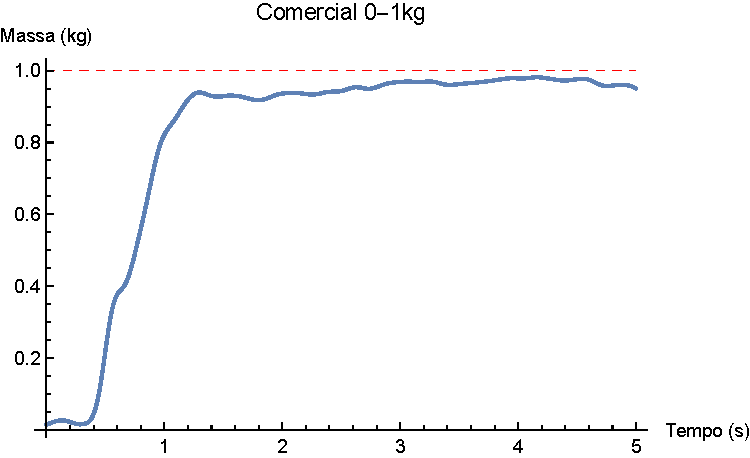
\includegraphics[width=\textwidth]{Comercial_0-1kg.pdf}
\caption{Curva temporal da resposta da célula de carga comercial quando adicionada uma carga de 1kg na célula em repouso.}
\label{fig:celula-comercial-resultado-0-1kg}
\end{figure}

Na Figura \ref{fig:celula-comercial-resultado-0-1kg} é possível observar que o tempo de resposta é baixo, de fato, nem é perceptível o tempo que ele leva para responder, uma vez que o fator mais notável no formato da curva não é a resposta do sensor nem da viga, mas a forma de como a carga era solta na viga. Era necessário segurar o peso para que a vibração do peso tivesse menor impacto na medida e este processo demorava aproximadamente 1 segundo, como pode ser visto na curva.

A Figura \ref{fig:celula-comercial-resultado-0-4kg} apresenta a resposta da célula quando adicionado um peso suspenso de $4 kg$ na barra. A curva foi filtrada por um filtro passa-baixas digital com frequência de corte de 5Hz para reduzir o efeito do ruído gerado pelo circuito de condicionamento.

\begin{figure}[H]
\center
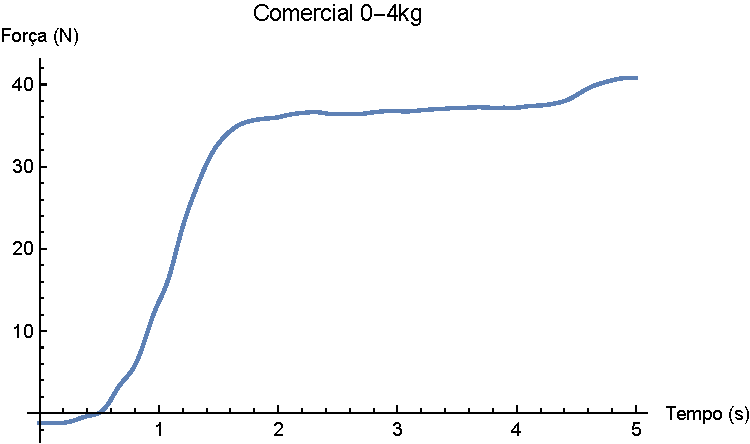
\includegraphics[width=\textwidth]{Comercial_0-4kg.pdf}
\caption{Curva temporal da resposta da célula de carga comercial quando adicionada uma carga de 4kg na célula em repouso.}
\label{fig:celula-comercial-resultado-0-4kg}
\end{figure}

A Figura \ref{fig:celula-comercial-resultado-0-4kg} é possível observar que a célula continua linear no intervalo de 4 kg e o valor de estabilidade da célula está muito próximo de 4kg ao final do tempo de 5 segundos. Entretanto, há um pequeno \textit{offset} no ponto de 0 kg que acredita-se ser devido a problemas no circuito de condicionamento. Esta hipótese não foi testada. A Figura \ref{fig:celula-comercial-resultado-0-4kg-etapa} apresenta um sistema equivalente ao da Figura \ref{fig:celula-comercial-resultado-0-4kg} contudo desta vez a massa foi adicionada em duas etapas, primeiramente somente 2kg foram suspensos e logo após mais uma segunda massa de 2kg foi suspensa, totalizando 4kg suspenso na viga. É possível ver claramente o tempo em que cada massa foi adicionada ao sistema.

\begin{figure}[H]
\center
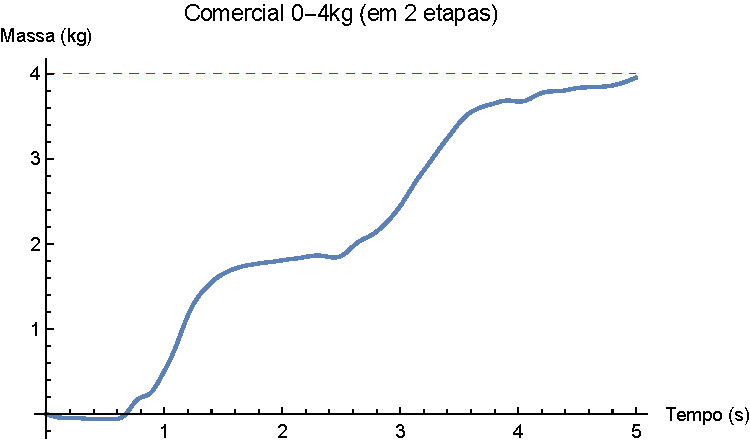
\includegraphics[width=\textwidth]{Comercial_0-4kg_etapa.pdf}
\caption{Curva temporal da resposta da célula de carga comercial quando adicionada uma carga de 4kg na célula em repouso em duas etapas (2kg + 2kg).}
\label{fig:celula-comercial-resultado-0-4kg-etapa}
\end{figure} 

A fim de validar a reprodutibilidade da célula, é necessário que a célula retorne ao ponto ponto de partida (0kg) quando as massas são removidas dos sistemas das Figuras \ref{fig:celula-comercial-resultado-0-4kg} e \ref{fig:celula-comercial-resultado-0-1kg}. A Figura \ref{fig:celula-comercial-resultado-1-0kg} apresenta a curva de resposta da célula quando uma carga de 1kg é removida.

\begin{figure}[H]
\center
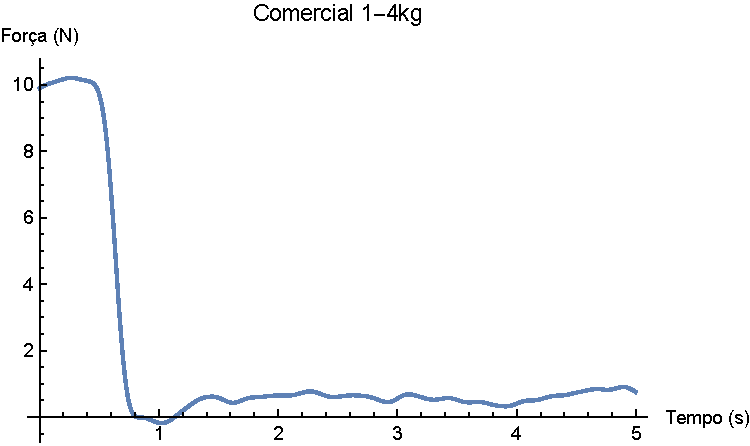
\includegraphics[width=\textwidth]{Comercial_1-0kg.pdf}
\caption{Curva temporal da resposta da célula de carga comercial quando se remove uma carga de 1kg.}
\label{fig:celula-comercial-resultado-1-0kg}
\end{figure}

Na Figura \ref{fig:celula-comercial-resultado-1-0kg} é possível observar que a resposta de remoção de carga é muito mais rápida do que a resposta de adição de carga, isto se dá ao fato de ser muito mais fácil (para o operador) remover a carga, pois basta que ele a eleve alguns centímetros ao invés de suspender onde ele deve ter cuidado para que não haja vibração que pode interferir com os resultados obtidos. Embora este efeito seja menos significante neste caso, ele ainda está presente em menor significância.

Outro fato interessante que é possível observar na Figura \ref{fig:celula-comercial-resultado-1-0kg} é o \textit{overshoot} presente ao redor da marca de 1 segundo. Acredita-se que este efeito é devido ao efeito elástico da viga, que ao ter a carga removida, se comporta como uma mola muito rígida e tem uma vibração muito rápida que logo se extingue devido à rigidez do material da célula de carga.

É possível dizer que a viga retornou ao valor inicial com a remoção da carga. É possível afirmar isto, pois a resolução de função de transferência medida foi de 0,2 kg e é possível observar que o valor final está ao redor do zero (isto é, está muito mais próximo do zero do que do 0,2kg).

A Figura \ref{fig:celula-comercial-resultado-4-0kg} apresenta a curva temporal de remoção de carga quando a viga está submetida a uma massa suspensa de 4kg e toda carga é removida de uma vez só.

\begin{figure}[H]
\center
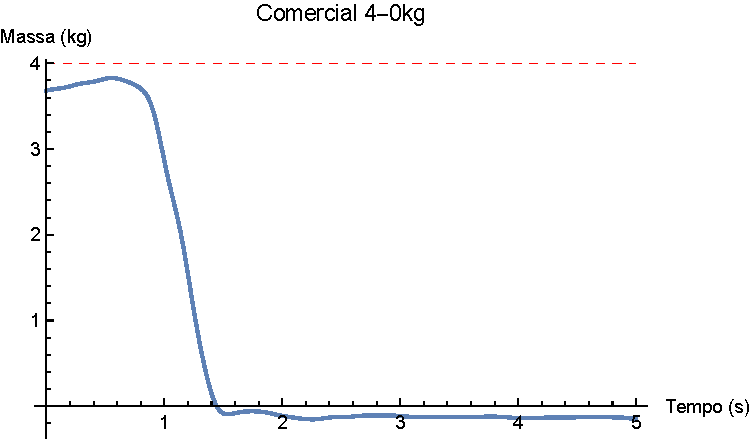
\includegraphics[width=\textwidth]{Comercial_4-0kg.pdf}
\caption{Curva temporal da resposta da célula de carga comercial quando se remove uma carga de 4kg.}
\label{fig:celula-comercial-resultado-4-0kg}
\end{figure}

Na Figura \ref{fig:celula-comercial-resultado-4-0kg} é menos visível o efeito elástico, embora este ainda esteja presente. Como na Figura \ref{fig:celula-comercial-resultado-1-0kg}, é possível afirmar que a célula retornou ao seu valor inicial e portanto o experimento teve sua reprodutibilidade confirmada.

\section{Célula de carga não-comercial}
A Tabela \ref{tab:celula-nao-comercial-resultado-funcao-transferencia} apresenta as medidas experimentais para a célula de carga não-comercial.


\begin{table}[H]
\centering
\caption{Tabela com os valores medidos experimentalmente para ajuste da função de transferência experimental da célula de carga não-comercial.}
\begin{tabular}{|l|l|l|}

\hline
\textbf{Massa (kg)} & \textbf{Tensão Elétrica (V)} & \textbf{Tensão Elétrica (V)} \\ \hline
 0.0 & 1.273 & 1.272 \\ \hline
 0.2 & 1.262 & 1.261 \\ \hline
 0.4 & 1.249 & 1.253 \\ \hline
 0.6 & 1.242 & 1.244 \\ \hline
 0.8 & 1.233 & 1.233 \\ \hline
 1.0 & 1.226 & 1.225 \\ \hline
\end{tabular}
\label{tab:celula-nao-comercial-resultado-funcao-transferencia}
\end{table}

A função que melhor ajusta os dados da Tabela \ref{tab:celula-nao-comercial-resultado-funcao-transferencia} é dada na Equação \ref{eq:celula-nao-comercial-resultado-funcao-transferencia}

\begin{equation}
	m(V) = 27.0883 - 21.309 V
	\label{eq:celula-nao-comercial-resultado-funcao-transferencia}
\end{equation}

\noindent onde $m(V)$ é a massa em $kg$ a qual a célula de carga está submetida e $V$ é a tensão elétrica em $volts$ medida na saída da ponte de Wheatstone com o sensor.

A função foi ajustada com $R^2$ dado pela Equação \ref{eq:celula-nao-comercial-resultado-funcao-transferencia-r2}. Já o erro de linearidade $\varepsilon_{L\%}$ encontrado devido à regressão foi de $7.33\%$.

\begin{equation}
	R^2 = 0.992582
	\label{eq:celula-nao-comercial-resultado-funcao-transferencia-r2}
\end{equation}

A sensibilidade observada experimentalmente para a célula de carga não comercial pode ser dada pela derivada da função de transferência experimental em razão da tensão elétrica, conforme a Equação \ref{eq:celula-nao-comercial-sensibilidade-experimental}

\begin{equation}
	S_{experimental}=\frac{d (m(V))}{d V }=-21.31\frac{Kg}{V} \textrm{ ou } S_{experimental}=-46.9\frac{mV}{Kg}
	\label{eq:celula-nao-comercial-sensibilidade-experimental}
\end{equation}

A Figura \ref{fig:celula-nao-comercial-resultado-funcao-transferencia} apresenta um gráfico com a função de transferência da Equação \ref{eq:celula-nao-comercial-resultado-funcao-transferencia} e os dados da Tabela \ref{tab:celula-nao-comercial-resultado-funcao-transferencia}.

\begin{figure}[H]
\center
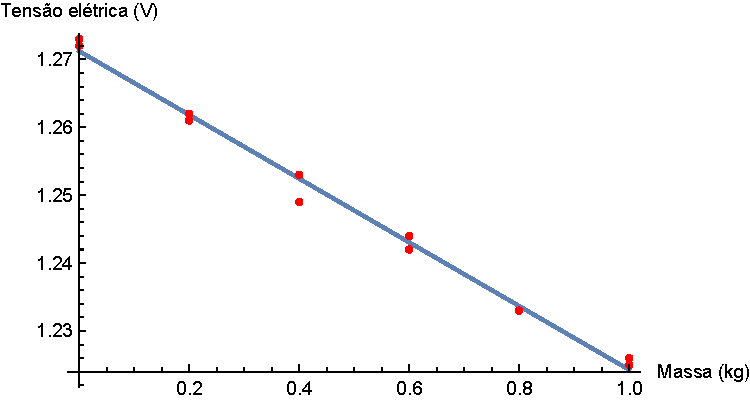
\includegraphics[width=\textwidth]{NaoComercial-Plot.pdf}
\caption{Função de transferência experimental: função de melhor ajuste e medidas experimentais}
\label{fig:celula-nao-comercial-resultado-funcao-transferencia}
\end{figure}

\noindent onde a linha contínua representa a função ajustada e os pontos representam cada medida individual realizada.

Na Figura \ref{fig:celula-nao-comercial-cadeia-medidas-experimental} pode-se verificar a cadeia de medidas experimental que foi executada para a célula de carga não comercial. \todo{informações de deformação de resistência dos SGs}

\begin{figure}[H]
\center
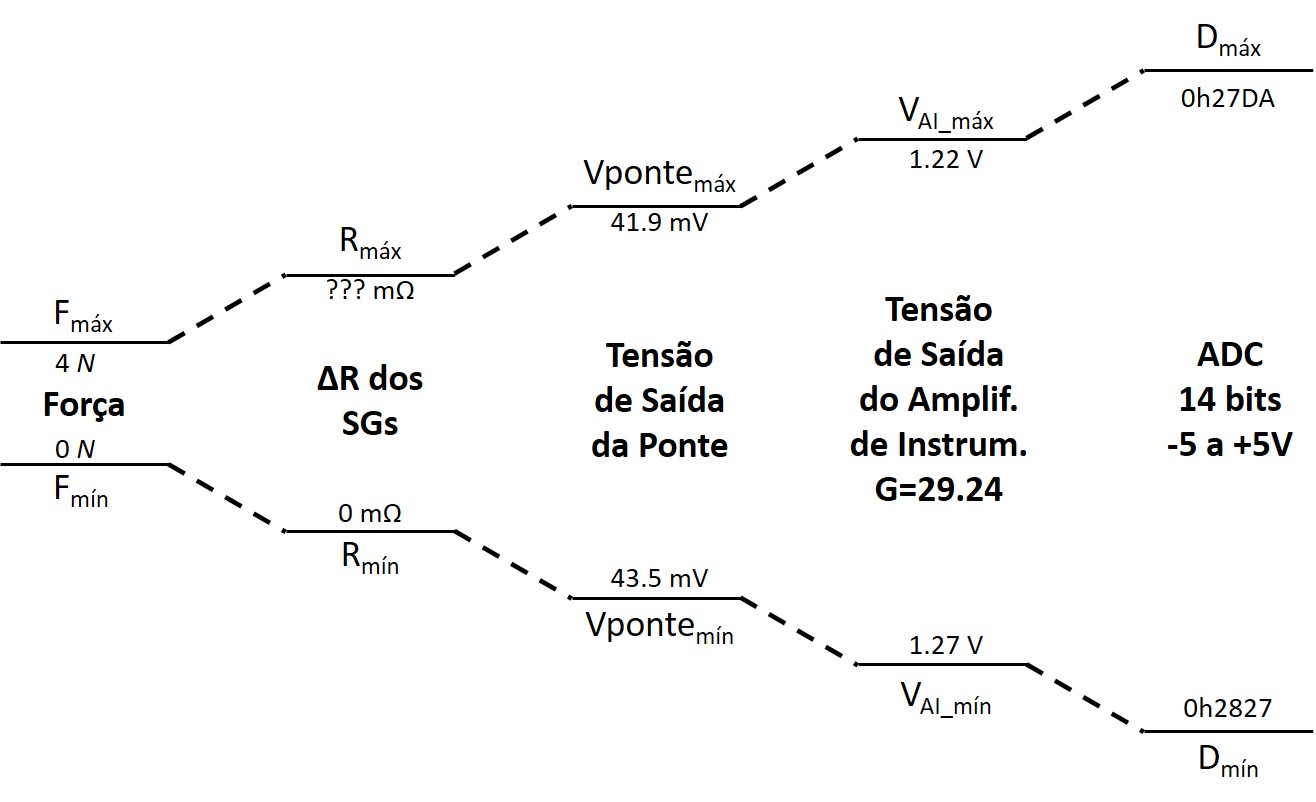
\includegraphics[width=0.7\textwidth]{CadeiaMedidasExperimental_CelulaNaoComercial.jpg}
\caption{Cadeia de medidas experimental executada para a célula de carga comercial}
\label{fig:celula-nao-comercial-cadeia-medidas-experimental}
\end{figure}

\subsection{Modelo computacional}

Os resultados obtidos por meio da modelagem computacional da célula de carga não comercial, na análise estática, para a tensão mecânica, deslocamento e deformação da célula para uma força aplicada de 4N são verificados a seguir.

Na Figura \ref{fig:celula-nao-comercial-computacional-tensao} é possível verificar que a maior tensão de Von Mises, ou tensão de cisalhamento, ocorre próximo ao ponto de engaste da viga.

\begin{figure}[H]
\center
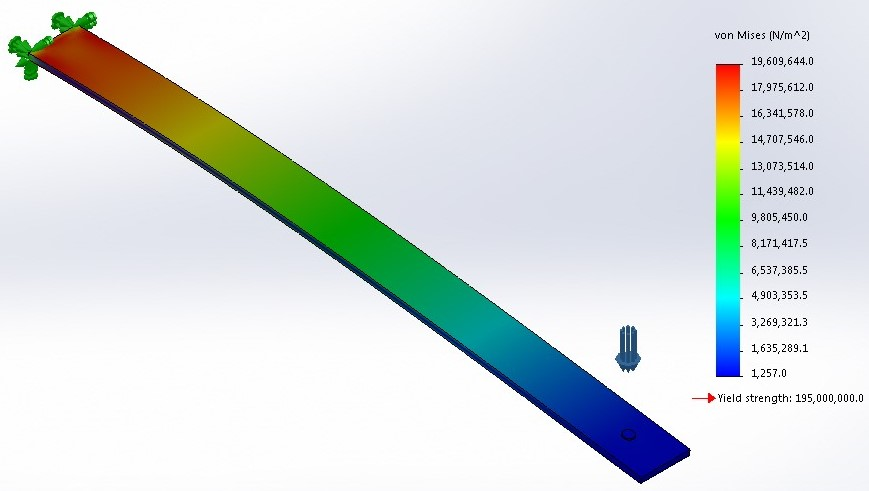
\includegraphics[width=0.7\textwidth]{CelulaNaoComercial_solid_tensao.jpg}
\caption{Resultado computacional para tensão de Von Mises para aplicação de 4N na célula não comercial}
\label{fig:celula-nao-comercial-computacional-tensao}
\end{figure}

Já a Figura \ref{fig:celula-nao-comercial-computacional-deslocamento} apresenta o deslocamento sofrido pela célula na simulação. Como era esperado, a parte de maior deslocamento ocorre na extremidade que está livre, no lado oposto ao engaste.

\begin{figure}[H]
\center
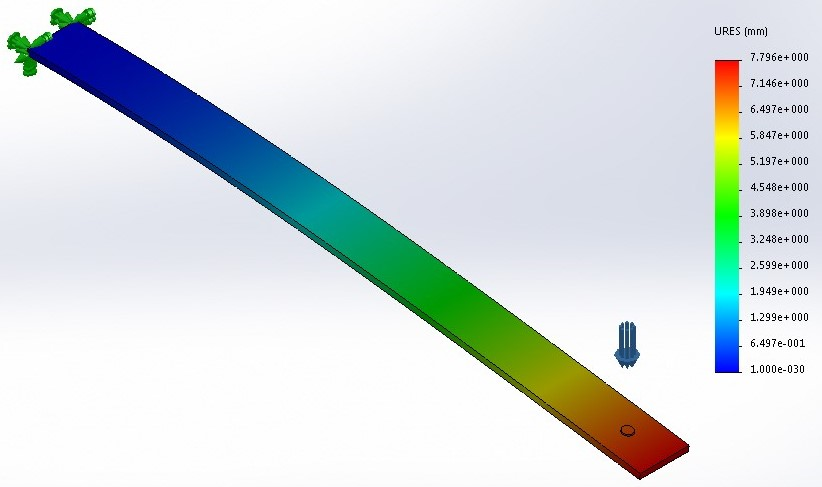
\includegraphics[width=0.7\textwidth]{CelulaNaoComercial_solid_deslocamento.jpg}
\caption{Resultado computacional para o deslocamento devido à aplicação de 4N na célula não comercial}
\label{fig:celula-nao-comercial-computacional-deslocamento}
\end{figure}

Quanto à deformação, a Figura \ref{fig:celula-nao-comercial-computacional-tensao} apresenta o resultado da simulação, na qual verifica-se que a região de maior deformação ocorre também próximo ao ponto de engaste da viga. Esta simulação é de extrema importância no estudo de montagens de células de cargas com o uso de extensômetros, pois esses devem ser colocados, sempre que possível, na região de maior deformação do material.

\begin{figure}[H]
\center
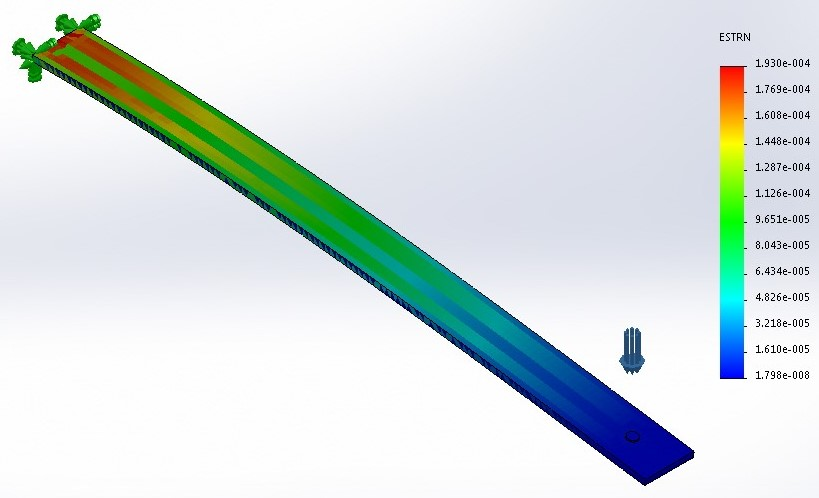
\includegraphics[width=0.7\textwidth]{CelulaNaoComercial_solid_deformacao.jpg}
\caption{Resultado computacional para a deformação devido à aplicação de 4N na célula não comercial}
\label{fig:celula-nao-comercial-computacional-deformacao}
\end{figure}

Na análise dinâmica em frequência da simulação computacional, foram analisados seus respectivos modos de vibração. A Tabela \ref{tab:celula-na-comercial-computacional-modos} apresenta os cinco primeiros modos de vibração observados pela simulação.

\begin{table}[H]
\centering
\caption{Modos de vibração resultantes da análise dinâmica da simulação computacional da célula não comercial}
\label{tab:celula-na-comercial-computacional-modos}
\begin{tabular}{|c|c|c|c|}
\hline
\textbf{Modo de Vibração} & \textbf{Rad/seg} & \textbf{Hz} & \textbf{Segundos} \\ \hline
1                         & 121.62           & 19.357      & 0.051662          \\ \hline
2                         & 762.15           & 121.3       & 0.008244          \\ \hline
3                         & 1027.9           & 163.59      & 0.0061129         \\ \hline
4                         & 2134.4           & 339.71      & 0.0029437         \\ \hline
5                         & 2813.8           & 447.83      & 0.002233          \\ \hline
\end{tabular}
\end{table}

Nas Figuras \ref{fig:celula-nao-comercial-computacional-modo1}, \ref{fig:celula-nao-comercial-computacional-modo2} e \ref{fig:celula-nao-comercial-computacional-modo3} é possível verificar os três primeiros modos de vibração simulados. Os resultados dos outros dois modos são um pouco exagerados e não cabem ser apresentados.

\begin{figure}[H]
\center
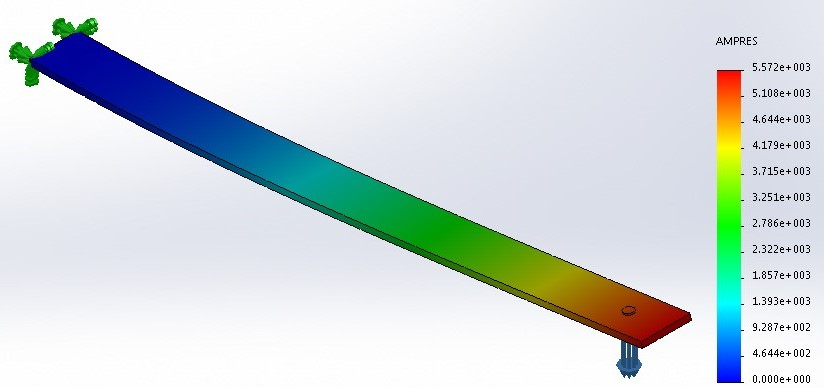
\includegraphics[width=0.7\textwidth]{CelulaNaoComercial_solid_modo1.jpg}
\caption{Resultado computacional para a deformação devido ao Modo de Vibração 1 na aplicação de 4N na célula não comercial}
\label{fig:celula-nao-comercial-computacional-modo1}
\end{figure}

\begin{figure}[H]
\center
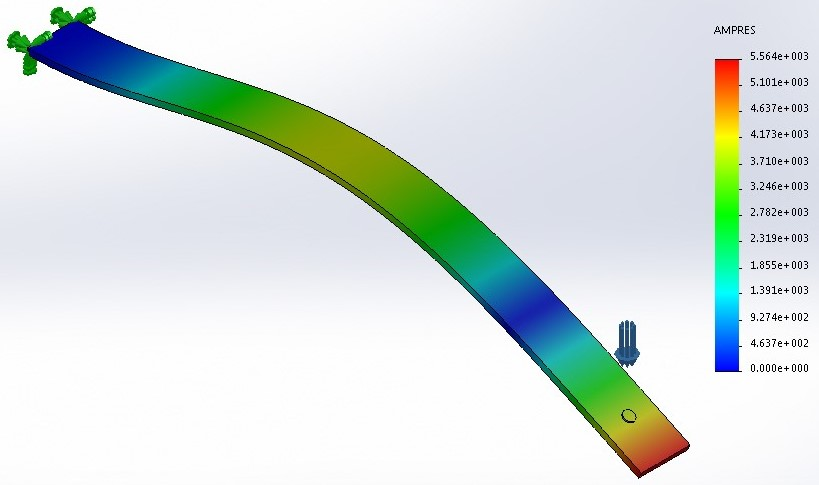
\includegraphics[width=0.7\textwidth]{CelulaNaoComercial_solid_modo2.jpg}
\caption{Resultado computacional para a deformação devido ao Modo de Vibração 2 na aplicação de 4N na célula não comercial}
\label{fig:celula-nao-comercial-computacional-modo2}
\end{figure}

\begin{figure}[H]
\center
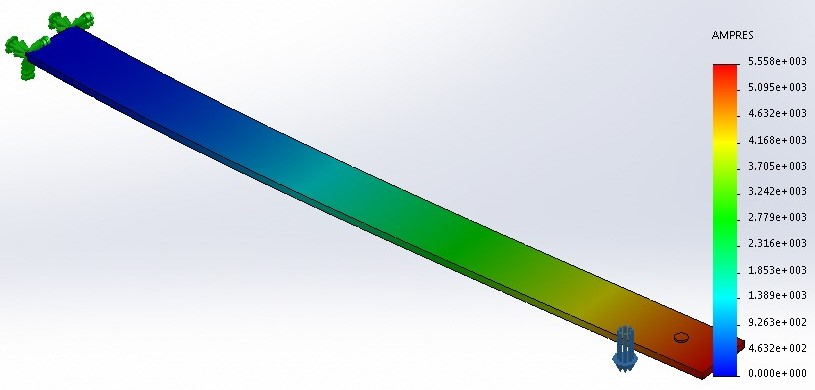
\includegraphics[width=0.7\textwidth]{CelulaNaoComercial_solid_modo3.jpg}
\caption{Resultado computacional para a deformação devido ao Modo de Vibração 3 na aplicação de 4N na célula não comercial}
\label{fig:celula-nao-comercial-computacional-modo3}
\end{figure}

A análise, tanto estática quanto dinâmica, da estrutura de uma célula de carga se faz importante para se poder mensurar alguns limites de trabalhos, verificar melhores pontos de aplicação de força e de deformação, e também para precaver quanto a futuros rompimentos da estrutura devido à  exposição nas suas frequências de ressonância.

\subsection{Resposta temporal}

Os resultados de resposta temporal no experimento realizado com a célula não comercial são apresentados e discutidos a seguir. Na Figura \ref{fig:celula-nao-comercial-resultado-0-400g} observa-se a inserção de uma massa de $400g$ na célula em repouso e sem carga. Nota-se que, em cerca de $1.8s$ a célula responde à alteração de carga, chegando a valores próximos da massa inserida. Uma pequena variação é percebida, e, por volta dos $3s$ o valor se estabiliza.

\begin{figure}[H]
\center
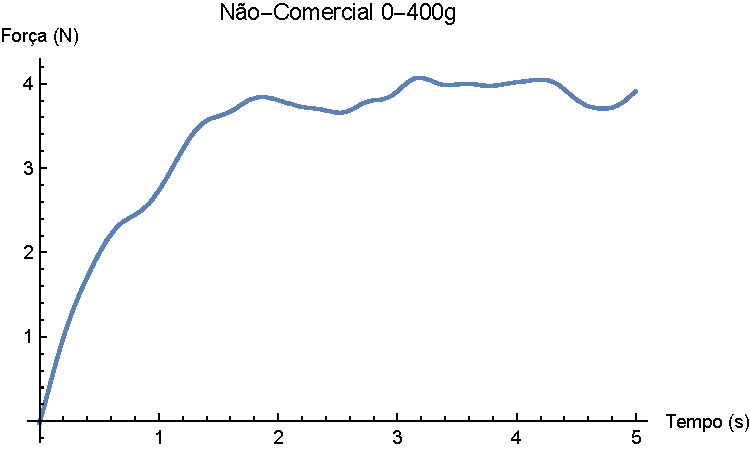
\includegraphics[width=\textwidth]{NaoComercial_0-400g.pdf}
\caption{Curva temporal da resposta da célula de carga não-comercial quando adicionada uma carga de 400g na célula em repouso.}
\label{fig:celula-nao-comercial-resultado-0-400g}
\end{figure}

Na avaliação temporal, com a inserção de $400g$ em duas etapas de $200g$, apresentada na Figura \ref{fig:celula-nao-comercial-resultado-0-400g-etapa}, nota-se que cada valor referencial foi atingido em cerca de $0.8s$, não havendo variações de tempo perceptíveis para a etapa $0-200g$ para a etapa $200-400g$.

\begin{figure}[H]
\center
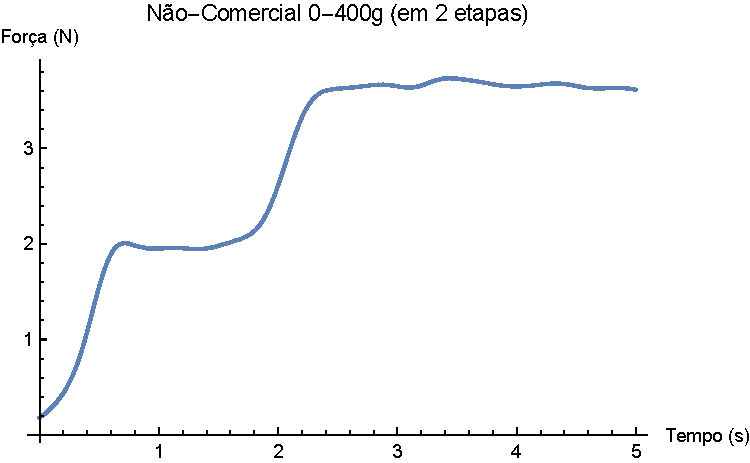
\includegraphics[width=\textwidth]{NaoComercial_0-400g_etapa.pdf}
\caption{Curva temporal da resposta da célula de carga não-comercial quando adicionada uma carga de 400g na célula em repouso em duas etapas (200g + 200g).}
\label{fig:celula-nao-comercial-resultado-0-400g-etapa}
\end{figure}

A Figura \ref{fig:celula-nao-comercial-resultado-0-1000g} apresenta a inserção, em uma única etapa, de $1000g$ na célula que estava em repouso e sem carga. Observa-se que, em aproximadamente $1.2s$, a curva atinge 95\% do seu valor referencial e, após $0.6s$, atinge a sua estabilidade.

\begin{figure}[H]
\center
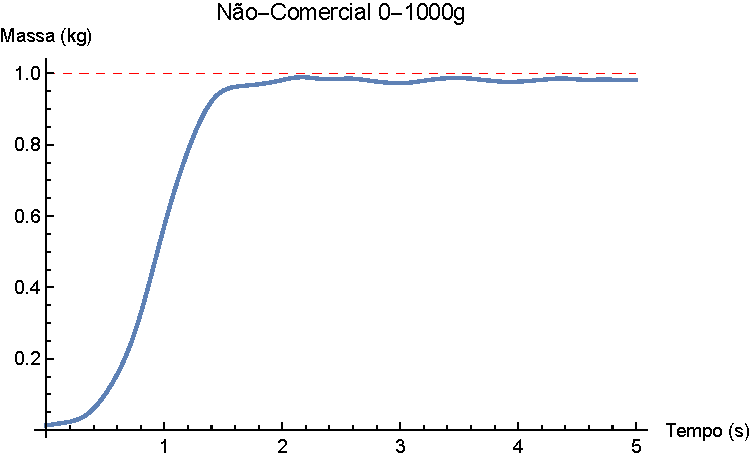
\includegraphics[width=\textwidth]{NaoComercial_0-1000g.pdf}
\caption{Curva temporal da resposta da célula de carga não-comercial quando adicionada uma carga de 1000g na célula em repouso.}
\label{fig:celula-nao-comercial-resultado-0-1000g}
\end{figure}

Na Figura \ref{fig:celula-nao-comercial-resultado-400-0g} verifica-se o efeito da retirada de uma carga de $400g$ da célula, em uma única etapa. Em menos de $1.0s$ o valor atinge o seu limite inferior, notando-se uma leve variação no sinal, devido à vibração remanescente da retirada da massa.

\begin{figure}[H]
\center
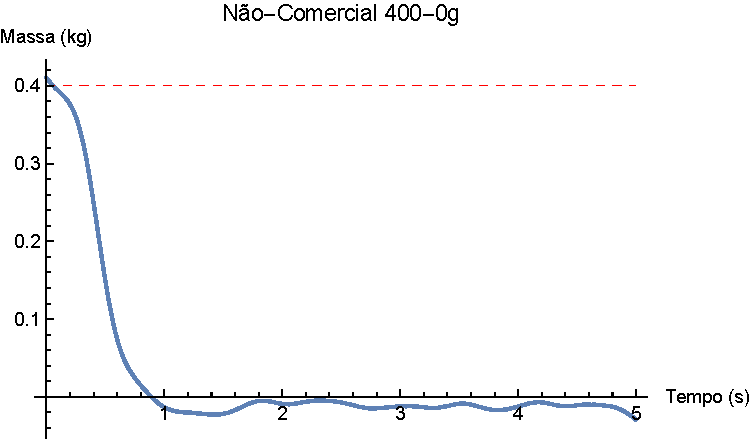
\includegraphics[width=\textwidth]{NaoComercial_400g-0.pdf}
\caption{Curva temporal da resposta da célula de carga comercial quando se remove uma carga de 400g.}
\label{fig:celula-nao-comercial-resultado-400-0g}
\end{figure}

O mesmo procedimento anterior foi então repetido, porém em duas etapas, retirando primeiramente $200g$ e, depois, os outros $200g$. O tempo que a curva leva para cada etapa é muito rápido, da ordem de $0.5s$, porém observa-se um valor residual no final, provavelmente em virtude do desgaste elástico do material da célula, conforme a Figura \ref{fig:celula-nao-comercial-resultado-400-0g-etapa}.

\begin{figure}[H]
\center
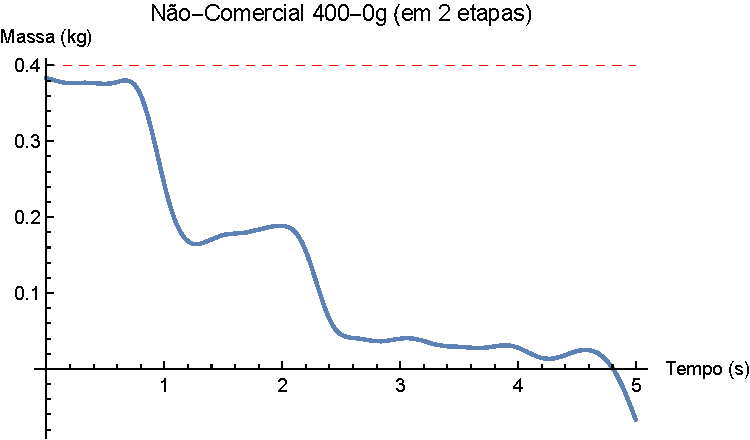
\includegraphics[width=\textwidth]{NaoComercial_400g-0_etapa.pdf}
\caption{Curva temporal da resposta da célula de carga comercial quando se remove uma carga de 400g em duas etapas (200g + 200g).}
\label{fig:celula-nao-comercial-resultado-400-0g-etapa}
\end{figure}

No caso da retirada de $1000Kg$ da célula, em uma única etapa, percebe-se um decaimento do sinal de forma muito rápida (cerca de $0.8s$), notando uma leve oscilação no final, como pode ser visto na Figura \ref{fig:celula-nao-comercial-resultado-1000-0g}.

\begin{figure}[H]
\center
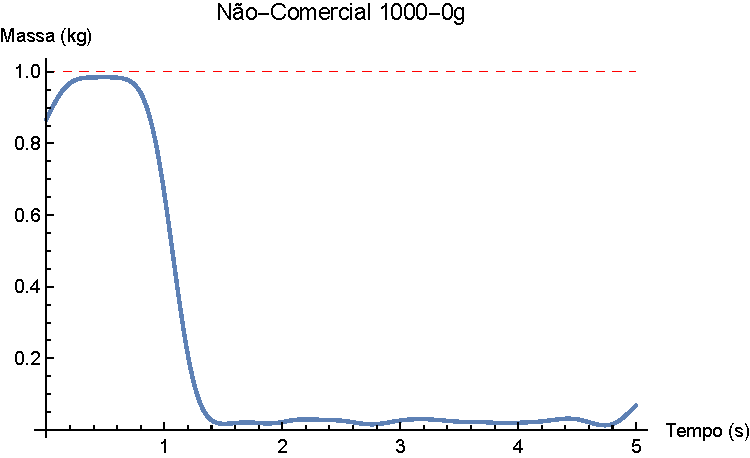
\includegraphics[width=\textwidth]{NaoComercial_1000g-0.pdf}
\caption{Curva temporal da resposta da célula de carga comercial quando se remove uma carga de 1000g.}
\label{fig:celula-nao-comercial-resultado-1000-0g}
\end{figure}

\subsection{Efeito do aquecimento da viga}

Como já mencionado, a célula utilizada está montada na configuração de meia ponte, porém com os dois extensômetros na mesma face da placa de metal, não fazendo assim a compensação por temperatura, que ocorreria caso um dos extensômetros estivesse na face superior e o outro na face inferior. Esta configuração é interessante para se observar o efeito térmico sobre os sensores. Ao aplicar uma chama de fogo a, aproximadamente, $10cm$ dos sensores, na face inferior da viga, por cerca de $4min$, percebeu-se uma variação na tensão de saída da ponte que, após processado o sinal e aplicada a função de transferência experimental já encontrada, notou-se uma variação da ordem de $0.5N$ que, considerando uma aceleração gravitacional $g$ de $10m/s^2$, corresponde a uma massa de $50g$. Esse resultado pode ser observado na Figura \ref{fig:celula-nao-comercial-resultado-aquecimento}.

\begin{figure}[H]
\center
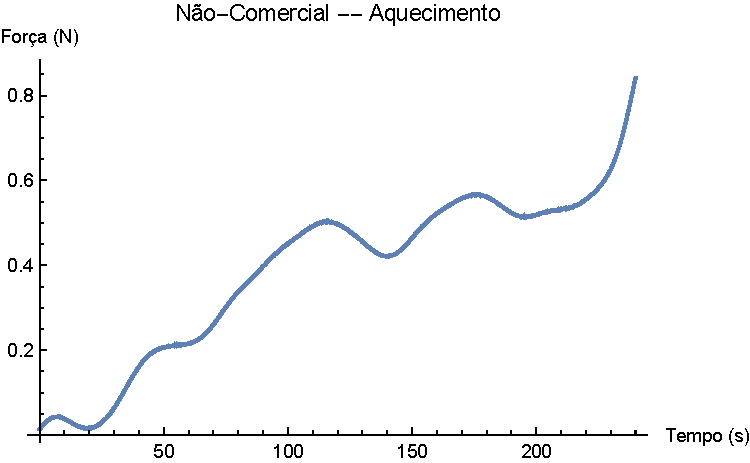
\includegraphics[width=\textwidth]{NaoComercial-Aquecimento.pdf}
\caption{Resposta temporal da célula de carga não-comercial para aquecimento de 4 minutos.}
\label{fig:celula-nao-comercial-resultado-aquecimento}
\end{figure}

\subsection{Análise da frequência fundamental}

Ao aplicar uma determinada força na viga, de forma muito rápida, captando a sua resposta no tempo, e aplicando uma \textit{Transformada de Fourier}, pode-se verificar a frequência fundamental de vibração da viga. A Figura \ref{fig:celula-nao-comercial-resultado-espectro} apresenta a magnitude do espectro das frequências observadas, percebendo-se um grande pico de magnitude por volta dos $20Hz$.

\begin{figure}[H]
\center
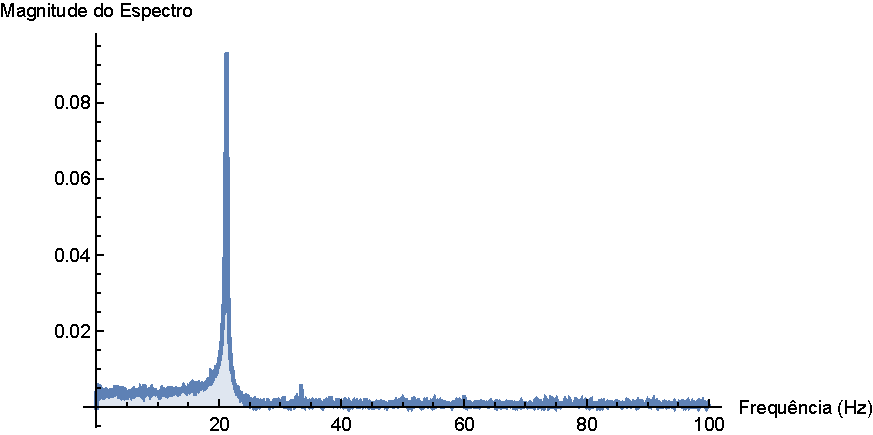
\includegraphics[width=\textwidth]{NaoComercial-Spectrum.pdf}
\caption{Espectro de frequência da célula de carga não-comercial quando submetida à uma batida. A curva de espectro foi suavizada por uma \textit{spline} de 3ª ordem.}
\label{fig:celula-nao-comercial-resultado-espectro}
\end{figure}

Na Figura \ref{fig:celula-nao-comercial-resultado-espectro-destaque} foi aplicado um \textit{zoom} no trecho próximo ao pico de magnitude percebido na Figura \ref{fig:celula-nao-comercial-resultado-espectro}. Com isso é possível estimar a frequência fundamental da viga, que é de, aproximadamente, $21.2Hz$. Valor esse compatível com o experimento feito na simulação computacional, que apontou $19.36Hz$ como frequência fundamental de vibração da viga. Já o segundo modo de vibração, que pela simulação computacional era de $121.3Hz$ não pôde ser observado, devido à sua baixa amplitude e o nível de ruído da amostragem, ficando por isso de fora faixa apresentada na Figura \ref{fig:celula-nao-comercial-resultado-espectro}

\begin{figure}[H]
\center
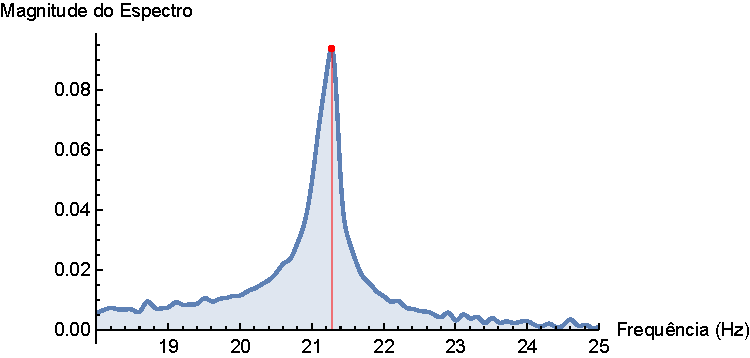
\includegraphics[width=\textwidth]{NaoComercial-SpectrumHighlight.pdf}
\caption{Destaque do espectro de frequência da célula de carga não-comercial (Figura \ref{fig:celula-nao-comercial-resultado-espectro}) quando submetida à uma batida e o pico máximo de frequência. A curva de espectro foi suavizada por uma \textit{spline} de 3ª ordem.}
\label{fig:celula-nao-comercial-resultado-espectro-destaque}
\end{figure}

\section{Torquímetro}
A Tabela \ref{tab:torquimetro-resultado-funcao-transferencia} apresenta as medidas experimentais para a célula de carga montada no torquímetro GEDORE FLEX-O-TORK Nº 4657.

\begin{table}[H]
\centering
\caption{Tabela com os valores medidos experimentalmente para ajuste da função de transferência experimental da célula de carga do torquímetro.}
\label{tab:torquimetro-resultado-funcao-transferencia}
\begin{tabular}{|c|c|}
\hline
\textbf{Torque ($lbf.ft$)} & \textbf{Tensão ($mV$)} \\ \hline
0                        & -101.1               \\ \hline
20                       & -73.4                \\ \hline
30                       & -65.3                \\ \hline
40                       & -64.3                \\ \hline
50                       & -53.6                \\ \hline
60                       & -44.7                \\ \hline
\end{tabular}
\end{table}

A função que melhor ajusta os dados da Tabela \ref{tab:torquimetro-resultado-funcao-transferencia} é dada na Equação \ref{eq:torquimetro-tf}.

\begin{equation}
	V(\tau) = -96.38 + 0.88 \tau
	\label{eq:torquimetro-tf}
\end{equation}
% em mv

\noindent onde $V(\tau)$ é a tensão em $mV$ a qual a célula de carga do torquímetro apresenta nos seus terminais de saída, ao estar submetida a um torque $\tau$, em $lbf.ft$. 

A função foi ajustada com $R^2$ dado pela Equação \ref{eq:torquimetro-tf-r2}. Já o erro de linearidade $\varepsilon_{L\%}$ encontrado devido à regressão foi de $15.13\%$, haja vista o experimento foi realizado com apenas uma repetição de amostras.

\begin{equation}
	R^2 = 0.954728
	\label{eq:torquimetro-tf-r2}
\end{equation}

O torquímetro apresentava também o seu cursor de indicação de torque em $N.m$, porém optou-se pela aquisição experimental em $lbf.ft$. Para realizar a conversão de $lbf.ft$ para $N.m$ pode-se utilizar a seguinte relação:

\begin{equation}
	1 lbf.ft = 1.3558 N.m
	\label{eq:torquimetro-relacao-unidades}
\end{equation}

A sensibilidade observada experimentalmente para a célula de carga do torquímetro pode ser dada pela derivada da função de transferência experimental em razão da tensão elétrica, conforme a Equação \ref{eq:torquimetro-sensibilidade-experimental}.

\begin{equation}
	S_{experimental}=\frac{d (V(\tau))}{d \tau }=0.88\frac{mV}{lbf.ft} \textrm{ ou } S_{experimental}=1.136\frac{lbf.ft}{mV}
	\label{eq:torquimetro-sensibilidade-experimental}
\end{equation}

A Figura \ref{fig:torquimetro-tf} apresenta um gráfico com a função de transferência da Equação \ref{eq:torquimetro-tf} e os dados da Tabela \ref{tab:torquimetro-resultado-funcao-transferencia}.

\begin{figure}[H]
\center
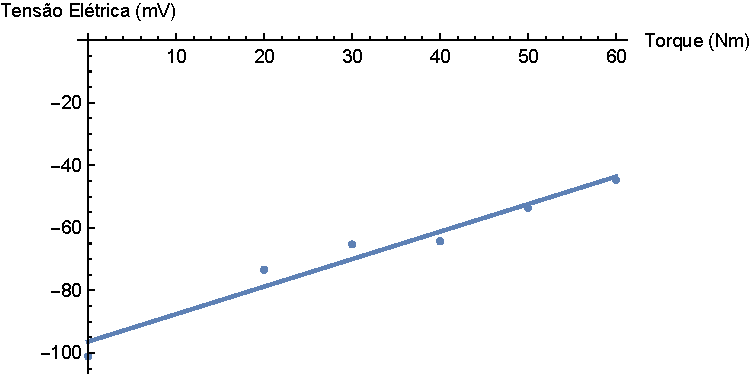
\includegraphics[width=\textwidth]{Torquimetro-Plot.pdf}
\caption{Função de transferência experimental do torquímetro e medidas experimentais}
\label{fig:torquimetro-tf}
\end{figure}

Na Figura \ref{fig:torquimetro-cadeia-medidas-experimental} pode-se verificar a cadeia de medidas experimental que foi executada para o torquímetro. Nota-se que não foi possível adquirir os valores de resistência elétrica dos extensômetros, haja vista se tratar de uma estrutura fechada, sem acesso a cada um dos sensores, estando disponível apenas os terminais da ponte interna.

\begin{figure}[H]
\center
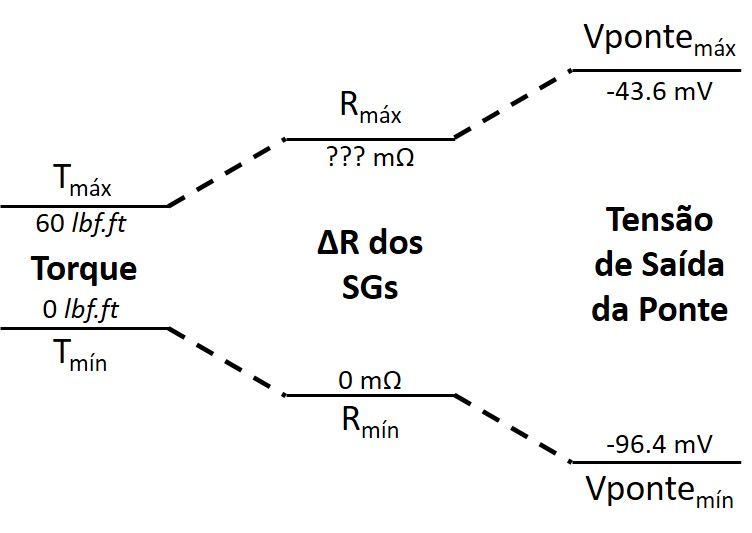
\includegraphics[width=0.7\textwidth]{CadeiaMedidasExperimental_Torquimetro.jpg}
\caption{Cadeia de medidas experimental executada para o torquímetro}
\label{fig:torquimetro-cadeia-medidas-experimental}
\end{figure}

\section{Análise de circuitos de condicionamento}

A Figura \ref{fig:condicionador-1} apresenta um circuito de condicionamento utilizando uma fonte de tensão de referência da Analog Devices (AD588) de 10V, ligada de forma a garantir uma corrente constante pela ponte. Porém esse circuito não oferece um ajuste de zero, necessário para esse tipo de aplicação.

\begin{figure}[H]
\center
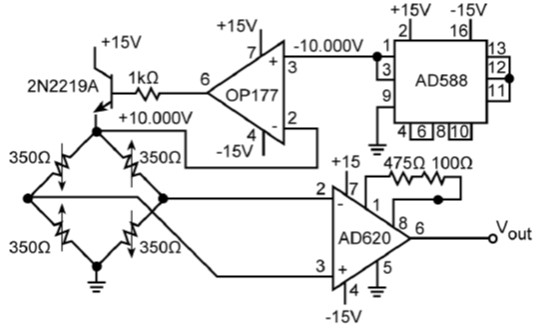
\includegraphics[width=0.7\textwidth]{condicionador_1.jpg}
\caption{Condicionador para uma ponte completa de 350$\Omega$}
\label{fig:condicionador-1}
\end{figure}

O circuito condicionador apresentado na Figura \ref{fig:condicionador-1} possui uma estrutura de alimentação da ponte, formada pelo AD588 e pelo amplificador operacional (OPAMP) OP177, formando uma fonte de corrente. O AD620 é um amplificador de intrumentação, com ganho dado pela Equação \ref{eq:ganho-AD620}.

\begin{equation}
	G=\frac{49.4k\Omega}{R}+1=\frac{49.4k\Omega}{575}+1=86.91
	\label{eq:ganho-AD620}
\end{equation}

Como solução para o ajuste de zero, propõe-se a inclusão de um potenciômetro multivoltas de 100k$\Omega$ ligado em suas extremidades às duas alimentações da fonte simétrica, e ligando o cursor a um resistor de 47k$\Omega$ até a entrada inversora do AD620. O potenciômetro proposto adiciona uma tensão de offset no terminar inversor do AD620, podendo assim regular a tensão.

Na Figura \ref{fig:condicionador-2} é apresentado um outro circuito de condicionamento, composto por um amplificador de instrumentação AD620B, um OPAMP AD705 e um conversor ADC.

\begin{figure}[H]
\center
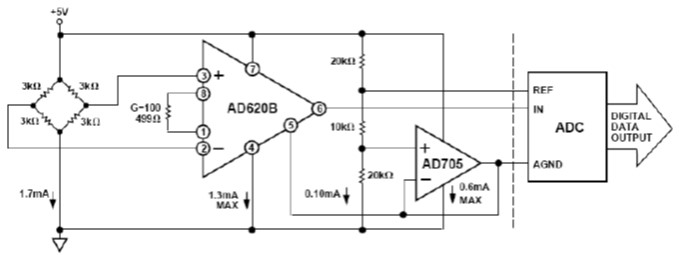
\includegraphics[width=0.7\textwidth]{condicionador_2.jpg}
\caption{Condicionador para uma ponte completa de 3k$\Omega$}
\label{fig:condicionador-2}
\end{figure}

A ponte é alimentada com uma tensão de +5V, tendo a sua saída diferencial amplificada pelo AD620B, com um ganho de 100. A saída do AD620B vai para a entrada do ADC. O OPAMP AD705 está montado numa configuração \textit{buffer}, com o seu terminal de entrada não inversor ligado a um divisor de tensão, fornecendo 2V nesse terminal. A saída do AD705 está ligada no terminal 5 do AD620B, denominada REF, que funciona como um offset para a saída em tensão do amplificador. Na entrada REF do ADC está ligada outra parte do divisor de tensão, fornecendo 3V. A saída do AD705, com 2V também está conectado à entrada AGND do ADC. De acordo com o \textit{datasheet} do AD620B \cite{datasheet-AD620}, muitos erros são evitados com a conexão feita desta forma.

O circuito apresentado na Figura \ref{fig:condicionador-2} é mostrado no próprio \textit{datasheet} do AD620B, mostrando esta configuração como um bom condicionador para aplicações de baixo custo, pois permite que o sistema sofra menos ruído com o GND virtual entre o ADC e o AD620B.

\chapter{Conclusões}

Foram realizados experimentos com três estruturas diferentes: uma célula de carga comercial, uma célula de carga não comercial, e uma célula de carga montada em um torquímetro. Tanto na célula de carga comercial como na não comercial foram montados circuitos de condicionamento do sinal, a fim de poder se fazer uma análise de melhor qualidade dos resultados experimentais.

Para a célula de carga comercial, por meio de um processo experimental de medidas, foram levantados valores para que se obtesse a função de transferência experimental, na faixa de $0Kg$ a $5Kg$, que representasse a resposta do sistema, para uma entrada em $Volts$ e uma saída em $Kg$. A função de transferência experimental encontrada apresentou um $R^2=0.998975$, um erro de linearidade $\varepsilon_{L\%}=3.09\%$ e uma sensibilidade $S_{exp}=-56.6\frac{mV}{Kg}$. Foram ainda feitos ensaios com a colocação e retirada de cargas na célula, na qual verificou-se a sua rapidez em atingir o valor correspondente à massa adicionada ou retirada.

Na célula de carga não comercial, primeiramente encontrou-se um problema para o condicionamento da configuração de ponte completa. Após verificar que os extensômetros da face inferior (compressão) estariam danificados, optou-se pela configuração de 1/2 ponte. Levantou-se então a função de transferência experimental, realizando medidas na faixa de $0g$ a $1000g$, com entrada em $Volts$ e saída em $Kg$. A função de transferência experimental apresentou um $R^2=0.992582$, um erro de linearidade $\varepsilon_{L\%}=7.33\%$ e uma sensibilidade $S_{exp}=-46.9\frac{mV}{Kg}$. Um dos motivo pelo qual encontrou-se um erro de linearidade alto pode ser a resolução de entrada um pouco elevada ($200g$), tendo em vista o \textit{range} escolhido ($0g$ a $1000g$). Para esta célula de carga ainda foi realizada uma simulação computacional utilizando o software SOLIDWORKS 2016, na qual pôde-se realizar uma análise estática, com verificação da tensão de cisalhamento, deslocamento e deformação para a aplicação de 4N de força na extremidade não engastada da viga, e também uma análise dinâmica, na qual verificam-se os 5 primeiros modos de vibração da viga simulada, tendo como frequência fundamental $19.36Hz$. Já na parte experimental prática, realizou-se uma análise da resposta temporal, com a adição e retirada de massas da extremidade da célula, verificando-se a rapidez da sua resposta perante a ação. Foi também realizado experimento para observar o efeito do aquecimento da viga, haja vista que a célula foi montada em configuração que não faz a compensação da variação da temperatura sobre os extensômetros. Após aproximadamente $4min$ de aplicação de calor há uma distância de cerca de $10cm$ dos sensores, verificou-se uma alteração nas resistências elétricas dos sensores que representou uma variação na ordem de $0.5N$ no valor de saída do sistema, como se houvesse a adição de cerca de $50g$ na extremidade livre da viga. Realizou-se também um experimento na qual verificou-se a frequência fundamental de vibração da viga, realizando uma batida e captando o sinal de saída. Com isso realizou-se uma \textit{Transformada de Fourier} e pôde-se verificar a frequência fundamental do sistema, que foi de $21.2Hz$, valor esse muito próximo do encontrado na simulação computacional.

No experimento realizado com a célula de carga montada em um torquímetro da marca GEDORE, na configuração de ponte completa, levantou-se a função de transferência experimental, tendo como entrada o torque, em $lbf.ft$, e saída em $mV$. O experimento foi realizado sem repetição, ou seja, uma única amostragem por valor de torque, razão essa que influenciou nos resultados da regressão linear para encontrar a função de transferência experimental, que apresentou um $R^2=0.954728$, um erro de linearidade $\varepsilon_{L\%}=15.13\%$ e uma sensibilidade $S_{exp}=0.88\frac{mV}{lbf.ft}$.

Ao final ainda foi realizada uma breve análise de alguns circuitos de condicionamento de sinal utilizados extensômetros.

Os experimentos realizados foram de grande valia para o aprendizado na aplicação, trabalho e condicionamento de extensômetros. Verificou-se que, por tratar de variações de resistência elétrica da ordem de $m\Omega$, é imprescindível um bom condicionamento do sinal para poder obter resultados com baixos níveis de erro. 

\newpage

\begin{thebibliography}{9}
\bibitem{mathematica-numerial-precision} \url{https://reference.wolfram.com/language/tutorial/NumericalPrecision.html}, acessado em 26 de abril de 2016
\bibitem{wikipedia-epsilon} \url{https://en.wikipedia.org/wiki/Machine_epsilon}, acessado em 26 de abril de 2016
\bibitem{livro-texto}  Balbinot, Alexandre; Brusamarello, Valner J., Instrumentação e Fundamentos de Medida - Vol.1 - 2ª Ed. Rio de Janeiro: LTC, 2014.
\bibitem{daq-specifications} NI USB-6009 -- DEVICE SPECIFICATIONS, \url{http://www.ni.com/pdf/manuals/375296a.pdf}, acessado em 3 de maio de 2016

\bibitem{daq-user-guide} NI USB-6009 -- USER GUIDE, \url{http://www.ni.com/pdf/manuals/371303n.pdf}, acessado em 3 de maio de 2016
\bibitem{datasheet-lm7805} Datasheet oferecido pelo fabricante do regulador de tensão elétrica LM7805CV, disponível em \url{http://www.datasheetlib.com/datasheet/221840/l7805cv_stmicroelectronics.html}.
\bibitem{datasheet-lm7905} Datasheet oferecido pelo fabricante do regulador de tensão elétrica LM7905, disponível em \url{http://www.ti.com/lit/ds/symlink/lm7905.pdf}.
\bibitem{datasheet-ref02} Datasheet oferecido pelo fabricante da referência de tensão elétrica REF02, disponível em \url{http://www.ti.com/lit/ds/sbvs003b/sbvs003b.pdf}.

\bibitem{datasheet-tl084} Datasheet oferecido pelo fabricante do amplificador operacional TL084, disponível em \url{http://www.ti.com.cn/cn/lit/ds/symlink/tl084.pdf}.

\bibitem{datasheet-ina126} Datasheet oferecido pelo fabricante amplificador de instrumentação INA126, disponível em \url{http://www.ti.com/lit/ds/symlink/ina126.pdf}.

\bibitem{datasheet-AD620} Datasheet oferecido pelo fabricante amplificador de instrumentação AD620, disponível em \url{http://pdf.datasheetcatalog.com/datasheet/analogdevices/105505445AD620_e.pdf}.


\end{thebibliography}

\iftoggle{attachments}{
	\chapter*{Anexos}
	\label{ch:attachments}
	\section{Mathematica}
	\todo{anexos do Mathematica}
}

\end{document}
